\documentclass{vcs_beamer}

\begin{document}

\author{Paul Cochrane}
\title[Version control with Git and Subversion]
        {Version control\\[0.2em]with Git and Subversion}
\date{\today}

\maketitle

%%%%%%%%%%%%%%%%%%%%%%%%%%%%%%%%%%%%%%%%%%%%%%%%%%%%%%%%%%%%%%%%%%%%%%%%%%%%
\begin{frame}
%\small
\begin{multicols}{2}
\begin{spacing}{0.8}
\tableofcontents
\end{spacing}
\end{multicols}
\end{frame}


%%%%%%%%%%%%%%%%%%%%%%%%%%%%%%%%%%%%%%%%%%%%%%%%%%%%%%%%%%%%%%%%%%%%%%%%%%%%
\section{About the course}

\subsection{Introduction and goals}
\begin{frame}{Introduction}
\begin{itemize}
    \item Any and all feedback is good
    \item Linux-focus; concepts are however usable everywhere
\end{itemize}

\onslide<2->{
{\Large \alert{Flow of course}}
\begin{itemize}
\item Version control in general
\item Git
\item Subversion
\item Server administration
\end{itemize}
}

\end{frame}

%%%%%%%%%%%%%%%%%%%%%%%%%%%%%%%%%%%%%%%%%%%%%%%%%%%%%%%%%%%%%%%%%%%%%%%%%%%%
\begin{frame}
\frametitle{Course goals}
that \ldots
\begin{itemize}
    \item more people use version control
    \item version control is used better
    \item one learns the basics of Git and Subversion
    \item one gets an impression of what is possible with these tools
    \item one obtains some experience in using the tools
\end{itemize}
\end{frame}

%%%%%%%%%%%%%%%%%%%%%%%%%%%%%%%%%%%%%%%%%%%%%%%%%%%%%%%%%%%%%%%%%%%%%%%%%%%%
\section{Cygwin installation}

%%%%%%%%%%%%%%%%%%%%%%%%%%%%%%%%%%%%%%%%%%%%%%%%%%%%%%%%%%%%%%%%%%%%%%%%%%%%
\begin{frame}
    \frametitle{Install Cygwin}
    \windowsframe

    \begin{itemize}
        \item Cygwin website: \url{http://www.cygwin.com}
        \item Download the \ttt{setup.exe} file
        \item Go to the folder containing this file and double click on it
        \item Click on \enquote{Next} a few times...
        \item Select \url{http://ftp.gwdg.de} as the download mirror
    \end{itemize}
\end{frame}

%%%%%%%%%%%%%%%%%%%%%%%%%%%%%%%%%%%%%%%%%%%%%%%%%%%%%%%%%%%%%%%%%%%%%%%%%%%%
\begin{frame}
    \frametitle{Install Cygwin (cont.)}
    \windowsframe

    \begin{itemize}
        \item Install the following packages:
            \begin{itemize}
                \item Devel $\rightarrow$ autoconf, automake, doxygen,
                    gcc4-fortran, gcc4-g++, make, subversion
                \item Net $\rightarrow$ openssh
                \item Perl $\rightarrow$ perl
                \item Publishing $\rightarrow$ texlive,
                    texlive-collection-basic,
                    texlive-collection-fontsrecommended,
                    texlive-collection-latex,
                    texlive-collection-latexextra,
                    texlive-collection-latexrecommended,
                    texlive-collection-pictures
                \item Python $\rightarrow$ python, python-tkinter
                \item X11 $\rightarrow$ fvwm, xinit, xorg-docs, xorg-server
            \end{itemize}
        \item Resolve dependencies (click on \enquote{Next})
        \item Ignore the \enquote{pango} error at the end and let the
            installer create a desktop icon and start menu item.
        \item Start the Cygwin terminal to set up the environment properly
    \end{itemize}
\end{frame}

% vim: expandtab shiftwidth=4:


%%%%%%%%%%%%%%%%%%%%%%%%%%%%%%%%%%%%%%%%%%%%%%%%%%%%%%%%%%%%%%%%%%%%%%%%%%%%
\section{Using the secure shell}

%%%%%%%%%%%%%%%%%%%%%%%%%%%%%%%%%%%%%%%%%%%%%%%%%%%%%%%%%%%%%%%%%%%%%%%%%%%%
\begin{frame}[fragile]
\frametitle{Server access via SSH}
\begin{itemize}
\item All project members have an account on the version control
    server (\ttalert{host.name}).
\item Your username is usually your last name
\item Access to the server is only possible via the secure shell (\ttalert{ssh})
\item Access is only possible with an ssh key
\end{itemize}
\end{frame}

%%%%%%%%%%%%%%%%%%%%%%%%%%%%%%%%%%%%%%%%%%%%%%%%%%%%%%%%%%%%%%%%%%%%%%%%%%%%
\begin{frame}[fragile]
\frametitle{SSH Passphrase}

A passphrase (as opposed to a password) makes \ttalert{ssh}-access to the
server much easier.  After one has entered the passphrase, it is possible to
access the server multiple times without having to enter the passphrase
again.  It isn't even necessary to enter your password!  However, a
passphrase is much longer (and therefore much harder to crack):
\begin{lstlisting}
Mary had a little lamb, its fleece was white as snow.
\end{lstlisting}

The secure shell uses \emph{public key encryption} which means that we need
to copy our public key to the remote server and then we can open an
encrypted connection.  We can then send data to and receive data from the
server over this connection.
\end{frame}

%%%%%%%%%%%%%%%%%%%%%%%%%%%%%%%%%%%%%%%%%%%%%%%%%%%%%%%%%%%%%%%%%%%%%%%%%%%%
\begin{frame}[fragile]
\frametitle{SSH Passphrase (cont.)}

Yes, but why?

\ttt{ssh} is a very good way to send data over a network.  It's a standard
method and it's secure.  It is, however, very annoying to have to enter
one's password each time a connection is made to the server, so a passphrase
makes data transfers and server connections transparent and easy.  Using a
passphrase with an encrypted connection makes using Subversion (and Git)
much, much easier.

To generate your private and public keys on Windows, you first need to
install PuTTY.
\end{frame}

% vim: expandtab shiftwidth=4:

%%%%%%%%%%%%%%%%%%%%%%%%%%%%%%%%%%%%%%%%%%%%%%%%%%%%%%%%%%%%%%%%%%%%%%%%%%%%
\begin{frame}
    \frametitle{Install PuTTY}
    \windowsframe

    \begin{itemize}
        \item Download PuTTY from
            \url{http://www.chiark.greenend.org.uk/~sgtatham/putty/download.html}
        \item Use the link under:
            \enquote{A Windows installer for everything except PuTTYtel}
        \item Double click on the installer and choose the default options
            in each window which appears when installing the software.
    \end{itemize}
\end{frame}

%%%%%%%%%%%%%%%%%%%%%%%%%%%%%%%%%%%%%%%%%%%%%%%%%%%%%%%%%%%%%%%%%%%%%%%%%%%%
\begin{frame}[fragile]
    \frametitle{Configure PuTTY}
    \windowsframe

    \begin{itemize}
        \item PuTTY Key Generator from Windows \enquote{Start Menu}
        \item Click on \enquote{Generate}
        \item Enter the passphrase and confirm
        \item Click on \enquote{Save private key}; save key as \ttt{host.ppk}
        \item Send the \enquote{Public key for pasting into OpenSSH
            authorized\_keys file} to \url{cochrane@}
    \end{itemize}
\end{frame}

%%%%%%%%%%%%%%%%%%%%%%%%%%%%%%%%%%%%%%%%%%%%%%%%%%%%%%%%%%%%%%%%%%%%%%%%%%%%
\begin{frame}[fragile]
    \frametitle{Configure PuTTY (cont.)}
    \windowsframe

    \begin{itemize}
        \item Start PuTTY from the Windows \enquote{Start Menu}
        \item Session $\rightarrow$
            Host name: \ttt{host.name}
        \item Connection $\rightarrow$ Data $\rightarrow$ Auto-login
            username: \ttt{your username}
        \item Connection $\rightarrow$ SSH $\rightarrow$ Auth $\rightarrow$
            Private key for authentication: \ttt{host.ppk}
        \item Session: Save
    \end{itemize}
\end{frame}

%%%%%%%%%%%%%%%%%%%%%%%%%%%%%%%%%%%%%%%%%%%%%%%%%%%%%%%%%%%%%%%%%%%%%%%%%%%%
\begin{frame}[fragile]
    \frametitle{Configure PuTTY (cont.)}
    \windowsframe

    \begin{itemize}
        \item Start \enquote{Pageant}
        \item Pageant can also be started at login time by adding a link to
            it in the user's \enquote{Startup} folder.
        \item Right-click on the Pageant icon $\rightarrow$ Add key
        \item Select \ttt{host.ppk} and type your passphrase (you only need
            to do this once every time you log on to Windows)
        \item Right-click on the Pageant icon $\rightarrow$ Saved sessions
            $\rightarrow$ \ttt{host.name}
        \item A console should appear with a prompt with your username and
            the name of the subversion server in it.
    \end{itemize}
\end{frame}

%%%%%%%%%%%%%%%%%%%%%%%%%%%%%%%%%%%%%%%%%%%%%%%%%%%%%%%%%%%%%%%%%%%%%%%%%%%%
\begin{frame}
    \frametitle{Notepad++ installation}
    \windowsframe
    \begin{itemize}
	\item Download Notepad++ from \url{http://notepad-plus-plus.org}
	\item Click on Agree, Next ... Install
    \end{itemize}

    \begin{itemize}
        \item We now have enough infrastructure in place that we can start
            talking about version control
    \end{itemize}
\end{frame}

% vim: expandtab shiftwidth=4:


%%%%%%%%%%%%%%%%%%%%%%%%%%%%%%%%%%%%%%%%%%%%%%%%%%%%%%%%%%%%%%%%%%%%%%%%%%%%
%%%%%%%%%%%%%%%%%%%%%%%%%%%%%%%%%%%%%%%%%%%%%%%%%%%%%%%%%%%%%%%%%%%%%%%%%%%%
\section{General version control concepts}

\begin{frame}{What is version control?}

\begin{description}
\item[Administrator] Organises and takes care of the history and different
    versions, trees and flows in a project (e.g. software development,
    document writing, server administration).
\item[Time machine] One can see and reinstate old states of files and entire
    projects.
\item[Quasi-backup] When the repository is kept on a separate server then
    this is basically a backup of the project.
\end{description}

\end{frame}


%%%%%%%%%%%%%%%%%%%%%%%%%%%%%%%%%%%%%%%%%%%%%%%%%%%%%%%%%%%%%%%%%%%%%%%%%%%%
\begin{frame}
\frametitle{Using version control}
{\large \alert{Who uses version control?}}

Everyone who would like to access an old version of a document.  Or everyone
to whom such things have happened:
\begin{itemize}
    \item \enquote{It would be nice to have the version from 2 hours ago \ldots}
    \item \enquote{I wrote that really well three days ago.  How did that go
        again?}
    \item \enquote{Oh no!  I deleted the file!}
\end{itemize}

{\large \alert{Where is version control used?}}
\begin{itemize}
\item Software development
\item Text and document processing/writing
\item Graphic design
\item System administration
\end{itemize}
\end{frame}

%%%%%%%%%%%%%%%%%%%%%%%%%%%%%%%%%%%%%%%%%%%%%%%%%%%%%%%%%%%%%%%%%%%%%%%%%%%%
\begin{frame}
\frametitle{Using version control (cont.)}
{\large \alert{What kinds of files should be kept under version control?}}

\begin{itemize}
\item Any kind of file which will be changed
\item Mainly text files
    \begin{itemize}
    \item Program code
    \item Documentation
    \item Theses, Dissertations
    \end{itemize}
\item But also binary files
    \begin{itemize}
    \item Graphics files; \ttalert{.png}, \ttalert{.tiff}
    \item Documents; \ttalert{.pdf}, \ttalert{.odt}
    \end{itemize}
\end{itemize}

{\large \alert{What shouldn't be kept under version control?}}

\begin{itemize}
\item Automatically generated files, e.g.: \ttalert{.o}, \ttalert{.log},
    \ttalert{.pdf}
\item Editor \enquote{backup} files, e.g.: \ttalert{file\~}, \ttalert{file.bak}
\end{itemize}

\end{frame}


%%%%%%%%%%%%%%%%%%%%%%%%%%%%%%%%%%%%%%%%%%%%%%%%%%%%%%%%%%%%%%%%%%%%%%%%%%%%
\begin{frame}[fragile]
\frametitle{Version control systems}
{\large \alert{Versions in file names}}

Does this look familiar?
\begin{lstlisting}
$ ls
file.1  file.20090803  file.keep  file.new  file.old.2
file.2  file.alt       file.neu   file.old
\end{lstlisting}

This is better than nothing, however what happened between the different
versions?  Which file is actually the most current?

{\large \alert{Automatic version control}}

There are many programs which can be used for the administration and
organisation of files:

\begin{itemize}
\item SCCS, RCS, CVS, Subversion, SVK, Git, Mecurial, Arch, Darcs, \ldots
\end{itemize}

\end{frame}


%%%%%%%%%%%%%%%%%%%%%%%%%%%%%%%%%%%%%%%%%%%%%%%%%%%%%%%%%%%%%%%%%%%%%%%%%%%%
\begin{frame}{Editing models}

\begin{itemize}
\item lock-modify-unlock  (RCS, also CVS, Subversion)
    \begin{itemize}
    \item File is checked out and locked; it can only be changed by one user
    \item File is modified
    \item File is checked in and unlocked
    \item \tbf{Disadvantage:} very inflexible
    \item \tbf{Advantage:} reduced effort when editing graphics files
    \end{itemize}
\item copy-modify-merge (CVS, Subversion, Git, \ldots)
    \begin{itemize}
    \item All files are copied from the repository and can be modified
        without restriction and independently of other copies
    \item When checking in modifications, the changes are automatically
        merged with other changes
    \item \tbf{Disadvantage:} Conflicts between changes can occur
    \item \tbf{Advantages:} very flexible; several people can work at the
        same time
    \end{itemize}
\end{itemize}

\end{frame}


%%%%%%%%%%%%%%%%%%%%%%%%%%%%%%%%%%%%%%%%%%%%%%%%%%%%%%%%%%%%%%%%%%%%%%%%%%%%
\begin{frame}{Repository models}

\begin{itemize}
\item Centralised Repository Model (client-server)
\end{itemize}
\begin{center}
    \resizebox{!}{0.7\textheight}{
        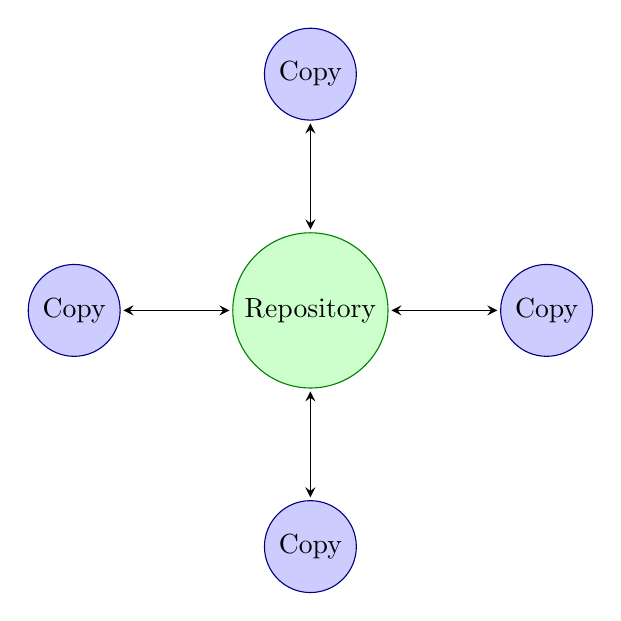
\begin{tikzpicture}
[repo/.style={circle,
		fill=green!20!white,
		draw=green!50!black,
		minimum size=10mm},
workingcopy/.style={circle,
		fill=blue!20!white,
		draw=blue!50!black,
		minimum size=5mm},
link/.style={<->, shorten <=1pt, shorten >=1pt, >=stealth, semithick}]

% central repo
\node at (0, 0) [repo] (mainrepo) { Repository };
% working copies
\node at (3,0)  [workingcopy] (copyright)  { Copy };
\node at (-3,0) [workingcopy] (copyleft)   { Copy };
\node at (0,3)  [workingcopy] (copytop)    { Copy };
\node at (0,-3) [workingcopy] (copybottom) { Copy };
% links between repo and working copies
\draw [link] (mainrepo) -- (copyright);
\draw [link] (mainrepo) -- (copyleft);
\draw [link] (mainrepo) -- (copytop);
\draw [link] (mainrepo) -- (copybottom);
\end{tikzpicture}

    }
\end{center}

\end{frame}

%%%%%%%%%%%%%%%%%%%%%%%%%%%%%%%%%%%%%%%%%%%%%%%%%%%%%%%%%%%%%%%%%%%%%%%%%%%%
\begin{frame}{Repository models (cont.)}

\begin{itemize}
\item Distributed Repository Model (pure); e.g. Linux Kernel
\end{itemize}
\begin{center}
    \resizebox{!}{0.7\textheight}{
        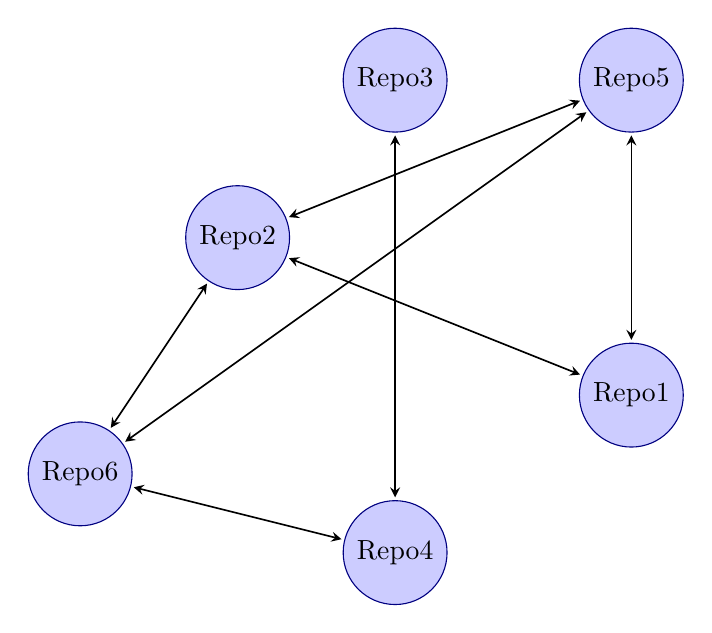
\begin{tikzpicture}
[repo/.style={circle,
		fill=green!20!white,
		draw=green!50!black,
		minimum size=10mm},
workingcopy/.style={circle,
		fill=blue!20!white,
		draw=blue!50!black,
		minimum size=5mm},
link/.style={<->, shorten <=1pt, shorten >=1pt, >=stealth, semithick}]

% central repo
%\node at (0, 0) [repo] (mainrepo) { Repository };
% working copies
\node at (3,-1)  [workingcopy] (repo1) { Repo1 };
\node at (-2,1)  [workingcopy] (repo2) { Repo2 };
\node at (0,3)   [workingcopy] (repo3) { Repo3 };
\node at (0,-3)  [workingcopy] (repo4) { Repo4 };
\node at (3,3)   [workingcopy] (repo5) { Repo5 };
\node at (-4,-2) [workingcopy] (repo6) { Repo6 };
% links between repos
\draw [link] (repo1) -- (repo2);
\draw [link] (repo1) -- (repo5);
\draw [link] (repo2) -- (repo5);
\draw [link] (repo3) -- (repo4);
\draw [link] (repo6) -- (repo2);
\draw [link] (repo6) -- (repo5);
\draw [link] (repo4) -- (repo6);
\end{tikzpicture}

    }
\end{center}

\end{frame}

%%%%%%%%%%%%%%%%%%%%%%%%%%%%%%%%%%%%%%%%%%%%%%%%%%%%%%%%%%%%%%%%%%%%%%%%%%%%
\begin{frame}{Repository models (cont.)}

\begin{itemize}
\item Distributed Repository Model (with a central server); e.g. Github
\end{itemize}
\begin{center}
    \resizebox{!}{0.7\textheight}{
        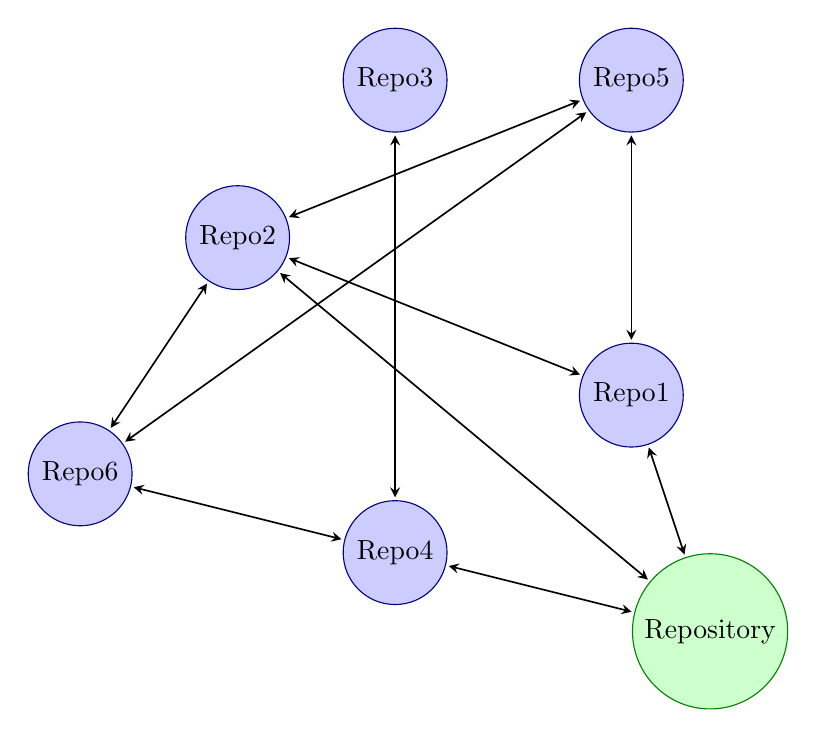
\begin{tikzpicture}
[repo/.style={circle,
		fill=green!20!white,
		draw=green!50!black,
		minimum size=10mm},
workingcopy/.style={circle,
		fill=blue!20!white,
		draw=blue!50!black,
		minimum size=5mm},
link/.style={<->, shorten <=1pt, shorten >=1pt, >=stealth, semithick}]

% working copies
\node at (3,-1)  [workingcopy] (repo1) { Repo1 };
\node at (-2,1)  [workingcopy] (repo2) { Repo2 };
\node at (0,3)   [workingcopy] (repo3) { Repo3 };
\node at (0,-3)  [workingcopy] (repo4) { Repo4 };
\node at (3,3)   [workingcopy] (repo5) { Repo5 };
\node at (-4,-2) [workingcopy] (repo6) { Repo6 };
% links between repos
\draw [link] (repo1) -- (repo2);
\draw [link] (repo1) -- (repo5);
\draw [link] (repo2) -- (repo5);
\draw [link] (repo3) -- (repo4);
\draw [link] (repo6) -- (repo2);
\draw [link] (repo6) -- (repo5);
\draw [link] (repo4) -- (repo6);
% central repo
\node at (4, -4) [repo] (mainrepo) { Repository };
% links to central repo
\draw [link] (mainrepo) -- (repo1);
\draw [link] (mainrepo) -- (repo2);
\draw [link] (mainrepo) -- (repo4);
\end{tikzpicture}

    }
\end{center}

\end{frame}

% vim: expandtab shiftwidth=4:

\documentclass{git_course}

\begin{document}

\author{Paul Cochrane}
\title[Version control with Git]
        {Version control with Git}
\date{\today}

\maketitle

\begin{frame}
\begin{multicols}{2}
\begin{spacing}{0.8}
\tableofcontents
\end{spacing}
\end{multicols}
\end{frame}


%%%%%%%%%%%%%%%%%%%%%%%%%%%%%%%%%%%%%%%%%%%%%%%%%%%%%%%%%%%%%%%%%%%%%%%%%%%%
\section{About the course}

\begin{frame}
\frametitle{Course Goals}

At the end of this course you should:

\begin{itemize}
    \item Feel comfortable using Git
    \item Know where to get further help, if necessary
    \item Be able to use Git on private projects
    \item Be able to collaborate with others using remote repositories
\end{itemize}
\end{frame}

\begin{frame}
\frametitle{Course Outline}
\begin{itemize}
    \item Introduction to Git and version control systems
    \item Installing Git
    \item Creating a first repository
    \item Getting help
    \item Tracking/staging/committing
    \item Configuring repositories
    \item General workflow
    \item Getting repository information
    \item Working with others
    \item Using branches and tags
    \item Rewriting history
    \item Contributing to Open Source projects
\end{itemize}
\end{frame}

\begin{frame}
\frametitle{Course Information}
\begin{itemize}
    \item Feedback most welcome
    \item Slides and notes are available on the GitHub docs site for the
        course:\\
        {\footnotesize \url{https://paultcochrane.github.io/version\_control\_course/}}
    \item You can submit pull requests, file issues, on GitHub:\\
        {\footnotesize \url{https://github.com/paultcochrane/version\_control\_course/}}
\end{itemize}
\end{frame}

\begin{frame}
\frametitle{About Me}
\begin{itemize}
    \item Physicist from New Zealand
    \item Have been involved in scientific computing and development of
        scientific software in Australia and Germany
    \item Led the scientific computing group at the Regional Computing
        Centre for Lower Saxony
    \item Currently a software developer for a startup in Bremen
        specialising in delivery of satellite-based information to users in
        polar regions
    \item Active in the Perl language community
\end{itemize}
\end{frame}


%%%%%%%%%%%%%%%%%%%%%%%%%%%%%%%%%%%%%%%%%%%%%%%%%%%%%%%%%%%%%%%%%%%%%%%%%%%%
\section{Version control systems and Git history}

\begin{frame}
\frametitle{What are Version Control Systems?}
\begin{itemize}
    \item A way to track changes to groups of files
    \item Most often used in software projects
    \item Most often used to track changes to text files (but not
        exclusively)
\end{itemize}
\end{frame}

\begin{frame}[fragile]
\frametitle{What are Version Control Systems?}
\begin{itemize}
    \item Akin to a time machine: one can return to previous states of a
        project
\end{itemize}
\begin{figure}
    \centerline{%
    \includegraphics[width=0.7\textwidth]{images/The_Delorian_William_Warby_flickr.pdf}}
        \caption{\tiny \emph{The Delorian}, by William Warby, Flickr:
    \url{https://www.flickr.com/photos/wwarby/9641216546/in/photostream/}}
\end{figure}
\end{frame}

\begin{frame}
\frametitle{What are Version Control Systems?}
\begin{itemize}
    \item Like a safety net: accidental file deletion isn't a catastrophe
        % -> image of a safety net
    \item Saved states are like anchor points in like rock climbing:
        one can fall back a small distance without losing everything
        % -> image of anchor point/rock climber
\end{itemize}
\end{frame}

\begin{frame}[fragile]
\frametitle{Why Use a Version Control System?}

Does this look familiar?

\begin{lstlisting}
file.1      file.20090803  file.keep
file.2      file.alt       file.old
file.old.2  file.fixed     file.new
\end{lstlisting}

This is better than nothing, however \ldots
\begin{itemize}
    \item what happened between the different versions?
    \item which file is actually the most current?
    \item what if \ttt{file.old} is the \emph{newest} file?
    \item can the differences between files tell us anything?
\end{itemize}
\end{frame}

\begin{frame}
\frametitle{Why Use a Version Control System?}
\begin{itemize}
    \item Useful in detecting when bugs were introduced or fixed
    \item Used to save known states of a group of files and hence versions
        (releases) of a software project
\end{itemize}
\end{frame}

\begin{frame}
\frametitle{Version Control Systems}
\begin{itemize}
    \item Local
        % -> image/diagram of local system
    \begin{itemize}
        \item e.g. RCS
    \end{itemize}
    \item Centralised
    \begin{center}
        \resizebox{!}{0.7\textheight}{
            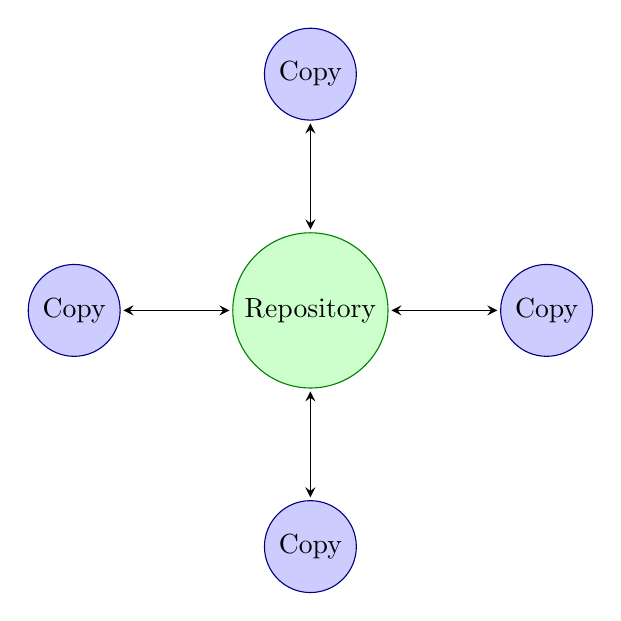
\begin{tikzpicture}
[repo/.style={circle,
		fill=green!20!white,
		draw=green!50!black,
		minimum size=10mm},
workingcopy/.style={circle,
		fill=blue!20!white,
		draw=blue!50!black,
		minimum size=5mm},
link/.style={<->, shorten <=1pt, shorten >=1pt, >=stealth, semithick}]

% central repo
\node at (0, 0) [repo] (mainrepo) { Repository };
% working copies
\node at (3,0)  [workingcopy] (copyright)  { Copy };
\node at (-3,0) [workingcopy] (copyleft)   { Copy };
\node at (0,3)  [workingcopy] (copytop)    { Copy };
\node at (0,-3) [workingcopy] (copybottom) { Copy };
% links between repo and working copies
\draw [link] (mainrepo) -- (copyright);
\draw [link] (mainrepo) -- (copyleft);
\draw [link] (mainrepo) -- (copytop);
\draw [link] (mainrepo) -- (copybottom);
\end{tikzpicture}

        }
    \end{center}
        % -> image/diagram of centralised system
    \begin{itemize}
        \item e.g. Subversion, CVS
    \end{itemize}
    \item Distributed
        % -> image/diagram of distributed system
    \begin{itemize}
        \item e.g. Git, Mercurial
    \end{itemize}
\end{itemize}
\end{frame}

\begin{frame}
\frametitle{Git History}
\begin{itemize}
    \item BitKeeper
    \item License problems
    \item Linux wrote his own system
    \item Open source
\end{itemize}
\end{frame}


%%%%%%%%%%%%%%%%%%%%%%%%%%%%%%%%%%%%%%%%%%%%%%%%%%%%%%%%%%%%%%%%%%%%%%%%%%%%
\section{Installing Git}

\begin{frame}
\frametitle{Installing Git (CLI options)}
\begin{itemize}
    \item Windows
    \item MacOS
    \item Linux/Unix
\end{itemize}
\end{frame}

\begin{frame}
\frametitle{Installing Git (GUI options)}
\begin{itemize}
    \item SourceTree
    \item TortoiseGit
\end{itemize}
\end{frame}

\begin{frame}
\frametitle{Use the Command Line}
\begin{itemize}
    \item With the command line one can get futher and do more; the
        learning curve is steeper, but it's worth it.
    \item Hence, we will focus on the command line interface (CLI) from now
        on.
\end{itemize}
    \blockquote[Hunt and Thomas, \emph{The Pragmatic Programmer}]
    {Gain familiarity with the shell, and you'll find your productivity soaring.}
\end{frame}

\begin{frame}
\frametitle{Text Editors}
\begin{itemize}
    \item Many options:
    \begin{itemize}
        \item Notepad++
        \item Vim, Emacs
        \item Atom
        \item Sublime text
    \end{itemize}
    \item We will be creating and editing text files, hence the need for a
        text editor.
    \item The choice of editor is unimportant; what \emph{is} important is
        that you feel comfortable using yours.
\end{itemize}
\end{frame}

%%%%%%%%%%%%%%%%%%%%%%%%%%%%%%%%%%%%%%%%%%%%%%%%%%%%%%%%%%%%%%%%%%%%%%%%%%%%
\section{Using Git on your own}

\begin{frame}
\frametitle{Using Git on your own}
\begin{itemize}
    \item Why?
    \item Get benefits of version control
    \item Get even more benefits when working with others; we'll discuss
        this in more detail later in the course
    \item Use Git on your local computer
\end{itemize}
\end{frame}

\begin{frame}
\frametitle{Starting a new repository from scratch}
\begin{itemize}
    \item mkdir something
    \item cd something
    \item git init  (also ls -la)
    \item git status
    \item create file
    \item git status (untracked)
    \item git add
    \item git status (staged)
    \item git commit
    \item git status (clean)
    \item git config user.name; git config user.email
    \item master is default branch
    \item (normally don't have to run git status all the time)
\end{itemize}
\end{frame}

\begin{frame}
\frametitle{Starting a new repository (conceptual steps)}
\begin{itemize}
    \item To create a repository, need to \ttt{init}ialise it
        \begin{itemize}
            \item git init
        \end{itemize}
    \item Repository is just a directory, with a .git directory
        \begin{itemize}
            \item ls -la
        \end{itemize}
    \item Things that go into a repository are just files
        \begin{itemize}
            \item touch file
        \end{itemize}
    \item To tell Git to track a file, need to \ttt{add} it
        \begin{itemize}
            \item git add
        \end{itemize}
    \item Tracked files and \emph{changes to tracked files} are put in
        the \emph{staging area}
        \begin{itemize}
            \item git status (see staged)
        \end{itemize}
    \item To record files and \emph{changes to files}, one \ttt{commit}s
        them to the repository
        \begin{itemize}
            \item git commit
        \end{itemize}
\end{itemize}
\end{frame}

\begin{frame}
\frametitle{Exercise: Start a new repository}
\begin{itemize}
    \item Repeat the previous steps on your own computer
    \item Create a directory and change into it
    \item Initialise the repository
    \item Run git status to see the current repository state
    \item Create a file (untracked); see the repository state
    \item Add the file to the repository (track it); see the repository state
    \item Commit the file to the repository; see the repository state
\end{itemize}
\end{frame}

\begin{frame}
\frametitle{Minor Detour: Git Configuration}
\begin{itemize}
    \item Brief intro to git config
    \item Repo-local config
    \item Global config
\end{itemize}
\end{frame}

\begin{frame}
\frametitle{Getting Help}
\begin{itemize}
    \item man pages
    \item git help
    \item books
    \item online references
\end{itemize}
\end{frame}

\begin{frame}
\frametitle{Exercise: git help}
\begin{itemize}
    \item Use \code{git help} on \code{init}, \code{add}, \code{commit} and
        \code{config} commands
    \item Open and browse on \url{https://git-scm.org}
\end{itemize}
\end{frame}

\begin{frame}
\frametitle{Parts of a local Git repository}
\begin{itemize}
    \item Working directory
    \item Staging area
    \item Repository
    \item Very important for understanding operations
    \item need image of wd, staging and repo
\end{itemize}
\end{frame}

\begin{frame}
\frametitle{Snapshots and diffs}
\begin{itemize}
    \item Photograph analogy
    \item Commits build on one another
    \item Working directory: checked out version of local repository
    \item Staging area: what will be committed next
    \item Repository: storage of snapshots
    \item Contrast with other systems, which store diffs between changes
\end{itemize}
\end{frame}

\begin{frame}
\frametitle{Basic workflow}
\begin{itemize}
    \item creation (mkdir, init, edit)
    \item saving snapshots of work (add, commit, return to edit step)
\end{itemize}
\end{frame}

\begin{frame}
\frametitle{Extending the sample project}
\begin{itemize}
    \item edit, add, commit
    \item seeing what we've done
    \begin{itemize}
        \item git log (--graph)
        \item git show
        \item git diff
    \end{itemize}
    \item deleting/renaming files
    \begin{itemize}
        \item git rm
        \item git mv
    \end{itemize}
\end{itemize}
\end{frame}

\begin{frame}
\frametitle{Explan SHAs}
\begin{itemize}
    \item in context of diff, show, log, etc.
\end{itemize}
\end{frame}

\begin{frame}
\frametitle{Exercise: extend the sample project further}
\begin{itemize}
    \item recommended steps \ldots
    \item practice git add/commit/rm/mv
    \item practice git log/show/diff
\end{itemize}
\end{frame}

\begin{frame}
\frametitle{Import existing project}
\begin{itemize}
    \item git init, git add, git commit
\end{itemize}
\end{frame}

\begin{frame}
\frametitle{Aliasing commands}
\begin{itemize}
    \item reduce typing, use alias
    \item handy aliases: st, di, ci, co
\end{itemize}
\end{frame}

\begin{frame}
\frametitle{Staging and unstaging files}
\begin{itemize}
    \item staging area in more depth
    \item unstage files one doesn't want to track
    \item git reset (just moves pointer/label)
\end{itemize}
\end{frame}

\begin{frame}
\frametitle{Exercise!}
\end{frame}

%%%%%%%%%%%%%%%%%%%%%%%%%%%%%%%%%%%%%%%%%%%%%%%%%%%%%%%%%%%%%%%%%%%%%%%%%%%%
\section{Using Git with others}

\begin{frame}
\frametitle{Working with others}
\begin{itemize}
    \item a networked world
    \item version control becomes more interesting when one works with
        others
    \item author and committer can be different people (usually aren't)
    \item work more often with branches (very powerful feature)
\end{itemize}
\end{frame}

\begin{frame}
\frametitle{Add remote repos to model}
\begin{itemize}
    \item working directory
    \item staging area
    \item local repo
    \item remote repo(s)
\end{itemize}
\end{frame}

\begin{frame}
\frametitle{Cloning an existing repo}
\begin{itemize}
    \item git clone
    \item changes to git config --list
    \item explain meaning of origin
    \item master, origin/master, HEAD
\end{itemize}
\end{frame}

\begin{frame}
\frametitle{Exercise!}
\end{frame}

\begin{frame}
\frametitle{Dealing with conflicts}
\begin{itemize}
    \item can happen when working on same part of a file
    \item happens when working with others
    \item happens when working with branches and stashes (hence can also
        happen when one is working alone!)
\end{itemize}
\end{frame}

\begin{frame}
\frametitle{Exercise!}
\end{frame}

\begin{frame}
\frametitle{Branches}
\begin{itemize}
    \item what are they?
    \item why use them?
    \item localise work on a focussed topic
    \item don't interfere with main development on master
    \item allows devs to work on parts of projects independently
    \item allows for code reviews before merging
\end{itemize}
\end{frame}

\begin{frame}
\frametitle{The default branch: master}

Discuss push/pull just from master?  Then have push/pull concept ready
for quick fix example below
\end{frame}

\begin{frame}
\frametitle{Branches}
\begin{itemize}
    \item git branch
    \item git branch -a
    \item git branch <branchname>
    \item git checkout <branchname>
    \item git checkout -b <branchname>
    \item naming branches -> clarity very helpful
\end{itemize}
\end{frame}

\begin{frame}
\frametitle{Simple branch}
\begin{center}
    \resizebox{!}{0.7\textheight}{
        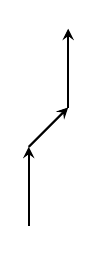
\begin{tikzpicture}
    [link/.style={->, >=stealth, thick}]

\draw [link] (0, 0) -- (0, 1);  % master
\draw [link] (0, 1) -- (0.5, 1.5);
\draw [link] (0.5, 1.5) -- (0.5, 2.5);  % branch

\end{tikzpicture}

    }
\end{center}
\end{frame}

\begin{frame}
\frametitle{Examples and exercises!}
\end{frame}

\begin{frame}
\frametitle{Merging branches}
\begin{itemize}
    \item merge changes on one branch into another
    \item git merge <branchname>
    \item fast-forward merge
    \item merge commits
    \item conflicts can occur (merge conflicts)
\end{itemize}
\end{frame}

\begin{frame}
\frametitle{Merging branches}
\begin{center}
    \resizebox{!}{0.7\textheight}{
        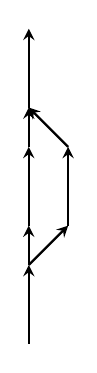
\begin{tikzpicture}
    [link/.style={->, >=stealth, thick}]

\draw [link] (0, 0) -- (0, 1);  % master
\draw [link] (0, 1) -- (0.5, 1.5);
\draw [link] (0.5, 1.5) -- (0.5, 2.5);  % branch
\draw [link] (0.5, 2.5) -- (0, 3);  % merge commit
\draw [link] (0, 3) -- (0, 4);

\draw [link] (0, 1) -- (0, 1.5);
\draw [link] (0, 1.5) -- (0, 2.5);
\draw [link] (0, 2.5) -- (0, 3);

\end{tikzpicture}

    }
\end{center}
\end{frame}

\begin{frame}
\frametitle{Example: quick fix}
\begin{itemize}
    \item when working on a new feature (on a feature branch)
    \item bug found on main branch -> quick fix necessary
    \item commit changes on current branch
    \item checkout master
    \item checkout quick fix branch (git checkout -b <branchname>)
    \item make fix, test, commit
    \item merge into master, push
    \item return to work on feature branch
\end{itemize}
\end{frame}

\begin{frame}
\frametitle{Example: handling merge conflicts}
\begin{itemize}
    \item work on same area of code
    \item try to merge
    \item handle (resolve) conflict
    \item git add (to mark as resolved)
    \item git commit (as necessary)
\end{itemize}
\end{frame}

\begin{frame}
\frametitle{Cherry picking}
\begin{itemize}
    \item associated with merging
    \item only when some commits are wanted
    \item git cherry-pick <commit>
\end{itemize}
\end{frame}

\begin{frame}
\frametitle{Local and remote branches}
\end{frame}

\begin{frame}
\frametitle{Fetching from remotes}
\begin{itemize}
    \item git pull $\approx$ git fetch; git merge
    \item why fetch then merge?
    \item origin is writable but upstream isn't -> common OSS model
    \item define upstream
    \item changes are made on upstream
    \item fetch changes to local repo
    \item merge changes into local branch (e.g. master)
\end{itemize}
\end{frame}

\begin{frame}
\frametitle{Exercise!}
\end{frame}

\begin{frame}
\frametitle{Rewriting history}
\begin{itemize}
    \item unpublished (not yet pushed) changes can be rearranged
    \item reorder, edit, squash, reword, delete (split also possible,
        but more involved)
    \item the story on wants to tell about the development; not all
        commits need to be pushed
    \item allows one to polish the changes; improve quality
    \item linearise changes; published repo has clear, linear history
        (see e.g. Ovid's slide about git histories)
\end{itemize}
\end{frame}

\begin{frame}
\frametitle{Interactive rebase}
\begin{itemize}
    \item git rebase -i
    \item very handy to clean up history before pushing
\end{itemize}
\end{frame}

\begin{frame}
\frametitle{Stashing changes}
\begin{itemize}
    \item why use this?
    \item what is this?
    \item handy feature for interrupted work
    \item e.g. quick fix example
    \item git stash
    \item git stash show -p
    \item git stash pop (conflicts possible)
    \item git stash drop
    \item git stash drop/show {n}
\end{itemize}
\end{frame}

%%%%%%%%%%%%%%%%%%%%%%%%%%%%%%%%%%%%%%%%%%%%%%%%%%%%%%%%%%%%%%%%%%%%%%%%%%%%
\section{Using a version control system service}

\begin{frame}
    \frametitle{Online VCS services}
    \begin{itemize}
        \item GitHub
        \item GitLab
        \item BitBucket
    \end{itemize}
\end{frame}

%%%%%%%%%%%%%%%%%%%%%%%%%%%%%%%%%%%%%%%%%%%%%%%%%%%%%%%%%%%%%%%%%%%%%%%%%%%%

https://stackoverflow.com/questions/953481/find-and-restore-a-deleted-file-in-a-git-repository

\begin{verbatim}
git checkout $(git rev-list -n 1 HEAD -- "$file")^ -- "$file"
\end{verbatim}

the file is then shown as a new file in the repo.  One can use `git diff
--cached` to see its contents.

\begin{verbatim}
git rev-list -n 1 HEAD -- "$file"
\end{verbatim}

finds the last commit affecting the file.  Since this is the last commit
affecting the file, it must be the commit where the file was deleted.  Hence
the commit directly preceding this one will be the last commit where the
file was still intact (the parent commit).  The parent commit of a given
commit is specified with the caret \ttt{\^} character, hence we check out
the parent commit of the deletion commit specifying just to operate on the
given file.
\end{document}

% vim: expandtab shiftwidth=4:

%%%%%%%%%%%%%%%%%%%%%%%%%%%%%%%%%%%%%%%%%%%%%%%%%%%%%%%%%%%%%%%%%%%%%%%%%%%%
\section{Subversion}

\begin{frame}
\begin{center}
\vspace{5em}
\Huge Subversion
\end{center}
\end{frame}

%%%%%%%%%%%%%%%%%%%%%%%%%%%%%%%%%%%%%%%%%%%%%%%%%%%%%%%%%%%%%%%%%%%%%%%%%%%%
\subsection{History}
\begin{frame}{Subversion---History}
\begin{itemize}
\item \href{http://en.wikipedia.org/wiki/Source_Code_Control_System}
           {SCCS--Source Code Control System}
    \begin{itemize}
    \item the first version control system
    \end{itemize}
\item \href{http://en.wikipedia.org/wiki/Revision_Control_System}
           {RCS--Revision Control System}
    \begin{itemize}
    \item free and more developed alternative to SCCS
    \item lock-modify-unlock
    \item basic functionality of version control
        \begin{itemize}
        \item checkout, checkin, log, diff
        \end{itemize}
    \item Decentralised Repository Model
    \end{itemize}
\item \href{http://en.wikipedia.org/wiki/Concurrent_Versions_System}
           {CVS--Concurrent Versions System}
    \begin{itemize}
    \item uses RCS as \enquote{backend}
    \item allows files to be changed at the same time
    \item many RCS operations in one go
    \item Client-Server model
    \item Centralised Repository Model
    \item became the standard tool for Open Source software development
    \item over time the design weaknesses became clear
    \end{itemize}
\end{itemize}
\end{frame}

%%%%%%%%%%%%%%%%%%%%%%%%%%%%%%%%%%%%%%%%%%%%%%%%%%%%%%%%%%%%%%%%%%%%%%%%%%%%
\begin{frame}{Subversion---History (cont.)}
\begin{itemize}
\item \href{http://en.wikipedia.org/wiki/Apache_Subversion}{SVN--Subversion}
    \begin{itemize}
    \item \enquote{a better CVS}; which is why it has a similar structure
	and \enquote{feel}
    \item Client-Server model
    \item Centralised Repository Model
    \item corrects many design weaknesses in CVS
    \item better support for binary files
    \item atomic commits
    \item reduced communication with the server
    \item files can be renamed and the history is retained
    \item \enquote{undo} is possible; \ttalert{svn revert}
    \item file properties
        \begin{itemize}
        \item executable
        \item binary/text
        \item keywords: \ttalert{Id}, \ttalert{Author},
            \ttalert{Revision} \ldots
        \end{itemize}
    \item became the standard tool in Open Source software development
    \end{itemize}
\end{itemize}
\end{frame}

%%%%%%%%%%%%%%%%%%%%%%%%%%%%%%%%%%%%%%%%%%%%%%%%%%%%%%%%%%%%%%%%%%%%%%%%%%%%
\subsection{Concepts and help}

\begin{frame}[fragile]
\frametitle{Subersion---Concepts}
\begin{itemize}
    \item Centralised repository model
    \item Client-Server model
\end{itemize}

{\large \alert{Working copies}}
\begin{itemize}
    \item One checks out a working copy on the client
    \item A working copy is just a copy of the files in the repository (on
	the server)
    \item Repository stays on the server
    \item It is possible to have multiple working copies checked out
\end{itemize}
\end{frame}

%%%%%%%%%%%%%%%%%%%%%%%%%%%%%%%%%%%%%%%%%%%%%%%%%%%%%%%%%%%%%%%%%%%%%%%%%%%%
\begin{frame}
\frametitle{Subversion---Concepts (cont.)}
{\large \alert{Directory structure}}

Subversion has a standardised directory structure:
\begin{description}
\item[trunk] The main development branch.  Often where the most work takes
    place.
\item[branches] Other lines of development.  Often used to work on new ideas
    and features so that development on the main branch isn't disturbed.
    Some projects work exclusively on branches and only very stable ideas
    and features make their way into the trunk.
\item[tags] Software releases often get \enquote{tagged} in order to give a
    state of development a human-friendly name.  Maintenance releases are
    sometimes developed further as a tag or a branch.
\end{description}
\end{frame}


%%%%%%%%%%%%%%%%%%%%%%%%%%%%%%%%%%%%%%%%%%%%%%%%%%%%%%%%%%%%%%%%%%%%%%%%%%%%
\begin{frame}[fragile]
\frametitle{Subversion---Help!}
\linuxframe

Help for all Subversion commands is available at the command line.  One
merely needs to use \ttalert{svn help}:
\begin{lstlisting}
svn help               # shows all commands
svn help <subcommand>  # shows help for the given command
\end{lstlisting}

For example:
\begin{lstlisting}[basicstyle=\tiny\ttfamily\color{black}]
$ svn help commit
commit (ci): Send changes from your working copy to the repository.
usage: commit [PATH...]

  A log message must be provided, but it can be empty.  If it is not
  given by a --message or --file option, an editor will be started.
  If any targets are (or contain) locked items, those will be
  unlocked after a successful commit.

Valid options:
  -q [--quiet]             : print nothing, or only summary information
  -N [--non-recursive]     : obsolete; try --depth=files or
--depth=immediates

 ...
\end{lstlisting}
\end{frame}

%%%%%%%%%%%%%%%%%%%%%%%%%%%%%%%%%%%%%%%%%%%%%%%%%%%%%%%%%%%%%%%%%%%%%%%%%%%%
\subsection{Importing, checking out and working}

\begin{frame}[fragile]
    \frametitle{Installing Subversion}
    \begin{itemize}
	\item Linux:
\begin{lstlisting}
$ sudo aptitude install subversion
\end{lstlisting}
	\item Windows:
	\begin{itemize}
	    \item Install Tortoise SVN
	    \item Download Tortoise SVN from
		\url{http://tortoisesvn.net/downloads.html}
	    \item Run the \ttt{.msi} file
	    \item Accept the license agreement
	    \item Install the command line tools
	    \item Next, Install...
	\end{itemize}
    \end{itemize}
\end{frame}

%%%%%%%%%%%%%%%%%%%%%%%%%%%%%%%%%%%%%%%%%%%%%%%%%%%%%%%%%%%%%%%%%%%%%%%%%%%%
\begin{frame}[fragile]
\frametitle{Steps to the first commit}
\linuxframe
\begin{itemize}
\item Import an existing project
    \begin{itemize}
    \item \ttalert{svn import}
    \item only happens the once for a repository
    \item and/or \ldots
    \end{itemize}
\item Check out an existing project
    \begin{itemize}
    \item \ttalert{svn checkout}
    \item can happen many times for one repository
    \item takes place after an \enquote{import}
    \item can also happen when no files are yet in the repository
    \item when one wants to take part in a project
    \item in order to see the source code of a project
    \end{itemize}
\item Now one can start work! \ttalert{:-)}
\end{itemize}
\end{frame}

%%%%%%%%%%%%%%%%%%%%%%%%%%%%%%%%%%%%%%%%%%%%%%%%%%%%%%%%%%%%%%%%%%%%%%%%%%%%
\begin{frame}[fragile]
\frametitle{Import a new project}
\linuxframe

Often the files for a project are already available.  Work has already taken
place on the project, but it isn't yet in version control.  For example,
this could be a software project to print \enquote{Hello world} to the
console.

Download the source files for the \enquote{hallo} project:
\begin{lstlisting}[basicstyle=\tiny\ttfamily\color{black}]
$ wget http://host.name/course_material/svn_git/hallo.tar.gz
$ tar -xvzf hallo.tar.gz
\end{lstlisting}

Here is a list of the files:
\begin{lstlisting}
$ ls hallo/
hallo.c  Makefile
\end{lstlisting}

One makes a new repository on the Subversion server with:
\begin{lstlisting}
$ svnadmin create /path/to/repo
\end{lstlisting}
This is normally done by the system administrator.

\end{frame}

%%%%%%%%%%%%%%%%%%%%%%%%%%%%%%%%%%%%%%%%%%%%%%%%%%%%%%%%%%%%%%%%%%%%%%%%%%%%
\begin{frame}[fragile]
\frametitle{Import a new project (cont.)}
\linuxframe

To import the \ttalert{hallo} project into Subversion, one uses the
\ttalert{svn import} command:
\begin{lstlisting}
$ svn import -m "<comment>" <directory> <repository URL>
\end{lstlisting}

\begin{lstlisting}[basicstyle=\tiny\ttfamily\color{black}]
$ svn import -m "Imported the hallo project" hallo/ \
    svn+ssh://vcskurs15@host.name/svnroot/userprojs/vcskurs15/hallo
Adding         hallo/hallo.c
Adding         hallo/Makefile

Committed revision 1.
\end{lstlisting}

The \ttalert{hallo} directory isn't yet a working copy.  We have only
imported the files into the repository.  In order to work on the project we
first need to check the project out from the repository with \ttalert{svn
checkout}.
\begin{lstlisting}
$ svn checkout <repository URL>/<project name> <working copy name>
\end{lstlisting}

\end{frame}

%%%%%%%%%%%%%%%%%%%%%%%%%%%%%%%%%%%%%%%%%%%%%%%%%%%%%%%%%%%%%%%%%%%%%%%%%%%%
\begin{frame}[fragile]
\frametitle{Import a new project (cont.)}
\linuxframe
However, before we check out the new project, we should move the old
\ttalert{hallo} directory to one side:
\begin{lstlisting}
$ mv hallo hallo_keep
\end{lstlisting}
We do this because we want to check out the working copy with the same name
as the imported directory.

Now we can check out the working copy.
\begin{lstlisting}[basicstyle=\tiny\ttfamily\color{black}]
$ svn checkout \
  svn+ssh://vcskurs15@host.name/svnroot/userprojs/vcskurs15/hallo hallo
A    hallo/hallo.c
A    hallo/Makefile
Checked out revision 1.
\end{lstlisting}

\end{frame}

%%%%%%%%%%%%%%%%%%%%%%%%%%%%%%%%%%%%%%%%%%%%%%%%%%%%%%%%%%%%%%%%%%%%%%%%%%%%
\begin{frame}[fragile]
\frametitle{Import a new project (cont.)}
\linuxframe

Now we can check if everything worked.  The standard Linux command
\ttalert{diff} shows the differences between the imported directory and the
checked out working copy.
\begin{lstlisting}
$ diff hallo hallo_keep
Only in hallo: .svn
\end{lstlisting}

The \ttalert{.svn} directory is a hidden directory (In Unix, directories
with names beginning with a dot are not normally shown.) where Subversion
keeps various administrative files.  For example, this is where the all
files in the main version of the repository are stored so that Subversion
doesn't need to connect to the server (and therefore doesn't need to use the
network) in order to carry out some basic tasks.

Keeping things clean is a good idea, hence we can now remove the old
directory:
\begin{lstlisting}
$ rm -r hallo_keep
\end{lstlisting}

\end{frame}

%%%%%%%%%%%%%%%%%%%%%%%%%%%%%%%%%%%%%%%%%%%%%%%%%%%%%%%%%%%%%%%%%%%%%%%%%%%%
\begin{frame}{Exercise---Import a new project}
\begin{itemize}
\item Download the \ttalert{hallo} example files
\item Import the directory into Subversion
\item Move the imported directory to one side
\item Check out a working copy
\item Compare the working copy with the old directory (\ttalert{diff})
\item Delete the old directory
\end{itemize}
\end{frame}

%%%%%%%%%%%%%%%%%%%%%%%%%%%%%%%%%%%%%%%%%%%%%%%%%%%%%%%%%%%%%%%%%%%%%%%%%%%%
\begin{frame}[fragile]
\frametitle{Solution---Import a new project}
\linuxframe
\begin{lstlisting}[basicstyle=\tiny\ttfamily\color{black}]
$ wget http://host.name/course_material/svn_git/hallo.tar.gz .
$ tar -xvzf hallo.tar.gz
$ svn import hallo/ svn+ssh://vcskurs15@host.name/svnroot/userprojs/vcskurs15/hallo \
    -m "Imported the hallo project"
$ mv hallo hallo_keep
$ svn checkout svn+ssh://vcskurs15@host.name/svnroot/userprojs/vcskurs15/hallo hallo
$ diff hallo hallo_keep
$ rm -r hallo_keep
\end{lstlisting}
\end{frame}

%%%%%%%%%%%%%%%%%%%%%%%%%%%%%%%%%%%%%%%%%%%%%%%%%%%%%%%%%%%%%%%%%%%%%%%%%%%%
\begin{frame}[fragile]
    \frametitle{Check out an existing project}
    \linuxframe
    \begin{itemize}
	\item The most common way to get the source code of a project, e.g.
        on Linux:
        \begin{itemize}
            \item Note that \ttalert{svn co} is another way of writing
                \ttalert{svn checkout}
        \end{itemize}
    \end{itemize}
\begin{lstlisting}[basicstyle=\tiny\ttfamily\color{black}]
$ svn co svn+ssh://vcskurs15@host.name/svnroot/userprojs/vcskurs15/hallo hallo
\end{lstlisting}
\end{frame}

%%%%%%%%%%%%%%%%%%%%%%%%%%%%%%%%%%%%%%%%%%%%%%%%%%%%%%%%%%%%%%%%%%%%%%%%%%%%
\begin{frame}
    \frametitle{Check out the project}
    \begin{itemize}
	\item In a Windows Explorer window navigate to
	    \ttt{C:$\backslash{}$cygwin$\backslash$home$\backslash$<username>},
	    right-click and select "SVN Checkout" in the menu which appears.
	\item URL of repository:
	    \ttt{svn+ssh://host.name/svnroot/repo.name}
	\item Click \enquote{OK}
	\item The source code for the project will now be checked out into the
	    given directory.
    \end{itemize}
\end{frame}

%%%%%%%%%%%%%%%%%%%%%%%%%%%%%%%%%%%%%%%%%%%%%%%%%%%%%%%%%%%%%%%%%%%%%%%%%%%%
\begin{frame}[fragile]
    \frametitle{Build the project}
    \begin{itemize}
	\item Now we're ready to build and develop the project!
	\item Start the Cygwin terminal
	\item Enter the project directory by typing the following:
	    \begin{lstlisting}
	    $ cd project.name
	    \end{lstlisting}
	\item Read the README (there are installation instructions in this
	    file):
	    \begin{lstlisting}
	    $ cat README
	    \end{lstlisting}
	\item Configure the project (only run once per checkout)
	    \begin{lstlisting}
	    $ autoreconf
	    $ ./configure
	    \end{lstlisting}
	\item Build and install the project (run whenever code has been
	    changed)
	    \begin{lstlisting}
	    $ make
	    $ make install
	    \end{lstlisting}
    \end{itemize}
\end{frame}

%%%%%%%%%%%%%%%%%%%%%%%%%%%%%%%%%%%%%%%%%%%%%%%%%%%%%%%%%%%%%%%%%%%%%%%%%%%%
\subsection{Commits}

\begin{frame}[fragile]
\frametitle{Commit concepts}

\begin{alertblock}{General concepts}
    \begin{itemize}
        \item most often used and perhaps most important operations in
            version control
        \item saves a given state of the project within the repository
        \item sometimes also referred to as a \emph{change}
            \begin{itemize}
                \item $\Rightarrow$ a commit is often compared to the
                    repository state at the previous commit
            \end{itemize}
    \end{itemize}
\end{alertblock}
\end{frame}

%%%%%%%%%%%%%%%%%%%%%%%%%%%%%%%%%%%%%%%%%%%%%%%%%%%%%%%%%%%%%%%%%%%%%%%%%%%%
\begin{frame}
    \frametitle{Commit concepts (cont.)}
    \begin{alertblock}{When should I commit something?}
        \vspace*{-4mm}
        \begin{itemize}
            \item that depends \ldots; here are my recommendations:
            \item when a small, complete \emph{idea} is finished, e.g. when
                \begin{itemize}
                    \item a new function has been written (also only a stub)
                    \item when a bug has been fixed; only check in code
                        fixing the bug
                \end{itemize}
            \item also: \enquote{when it makes sense}
            \item small commits are easier for humans to understand
            \item teamwork: commits give the possiblity to give and receive
                feedback about your contributions.  Problems can therefore
                be found and corrected earlier.  Large commits stop others
                from checking what you did (and what you did could contain
                major errors!).
        \end{itemize}
    \end{alertblock}
    \vspace*{-5mm}
    See also:
    \begin{itemize}
            \tiny
        \item \url{http://sethrobertson.github.io/GitBestPractices}
        \item \url{http://blog.looplabel.net/2008/07/28/best-practices-for-version-control};
            items 4 and 5
            \normalsize
    \end{itemize}
\end{frame}

%%%%%%%%%%%%%%%%%%%%%%%%%%%%%%%%%%%%%%%%%%%%%%%%%%%%%%%%%%%%%%%%%%%%%%%%%%%%
\begin{frame}[fragile]
    \frametitle{Commit concepts (cont.)}
    \begin{alertblock}{How often should I commit?}
        \begin{itemize}
            \item as often as possible
            \item \enquote{release early, release often}
            \item as soon as the changes belonging to a given idea are finished
            \item don't be afraid to commit!
        \end{itemize}
    \end{alertblock}
\end{frame}

%%%%%%%%%%%%%%%%%%%%%%%%%%%%%%%%%%%%%%%%%%%%%%%%%%%%%%%%%%%%%%%%%%%%%%%%%%%%
\begin{frame}[fragile]
\frametitle{Commit messages}

\begin{itemize}
    \item Each commit needs a \enquote{commit message} describing the change
    \item Commit messages document what was done in each change and \emph{why}
    \item An important part of communication within a project:
        \begin{itemize}
            \item commit logs are messages to other people
            \item \ldots and are messages to yourself in the future!
        \end{itemize}
\end{itemize}

\begin{alertblock}{What should I write in a commit message?}
    \vspace*{-4mm}
    \begin{itemize}
        \item a short description of the change
        \item the description can sometimes be longer than the actual
            change!  The message describes the \enquote{why} of the change.
        \item the message should be able to explain later what happened in
            the change
        \item note: when problems occur, this is where one looks first for
            information
    \end{itemize}
\end{alertblock}
\vspace*{-5mm}
\begin{center}
{\large
    Commit messages such as \lstinline{Added some code.} don't help
    \emph{anyone}!
}
\end{center}

\end{frame}

%%%%%%%%%%%%%%%%%%%%%%%%%%%%%%%%%%%%%%%%%%%%%%%%%%%%%%%%%%%%%%%%%%%%%%%%%%%%
\begin{frame}[fragile]
    \linuxframe
    \frametitle{Let's finally commit something!}
    \begin{itemize}
        \item To commit something, first we need to change something
        \item Change the \ttalert{hallo.c}
        \item Build the program
\begin{lstlisting}
$ make
\end{lstlisting}
        \item Does the program still work?
\begin{lstlisting}
./hallo
\end{lstlisting}
        \item Check the status of the working copy
        \begin{itemize}
            \item \ttalert{svn status} or \ttalert{svn st}
        \end{itemize}
\begin{lstlisting}
$ svn status
M      hallo.c
?      hallo
\end{lstlisting}
        \item We'll take care of the generated \ttalert{hallo} file later
    \end{itemize}
\end{frame}

%%%%%%%%%%%%%%%%%%%%%%%%%%%%%%%%%%%%%%%%%%%%%%%%%%%%%%%%%%%%%%%%%%%%%%%%%%%%
\begin{frame}[fragile]
    \frametitle{Let's finally commit something!}
    \begin{itemize}
        \item To commit something, first we need to change something
        \item Open Windows Explorer
        \item Navigate to
            \ttalert{C:\T{}cygwin\T{}home\T{}<username>\T{}project.name\T{}trunk\T{}devel\T{}vcs\_course}
        \item Open the file \ttalert{hallo.f90} in \notepad
        \item Change the \ttalert{hallo.f90}
        \item Build the program (in Cygwin)
\begin{lstlisting}
$ make
\end{lstlisting}
        \item Does the program still work? (Cygwin)
\begin{lstlisting}
./hallo
\end{lstlisting}
    \end{itemize}
\end{frame}

%%%%%%%%%%%%%%%%%%%%%%%%%%%%%%%%%%%%%%%%%%%%%%%%%%%%%%%%%%%%%%%%%%%%%%%%%%%%
\begin{frame}
    \frametitle{Let's finally commit something! (cont.)}
    \begin{itemize}
        \item The status of the working copy has changed
            \begin{itemize}
                \item The green tick has changed to a red exclamation mark
            \end{itemize}
        \item We'll take care of the generated \ttalert{hallo} file later
            (denoted by the blue question mark)
    \end{itemize}
    \centering{
        %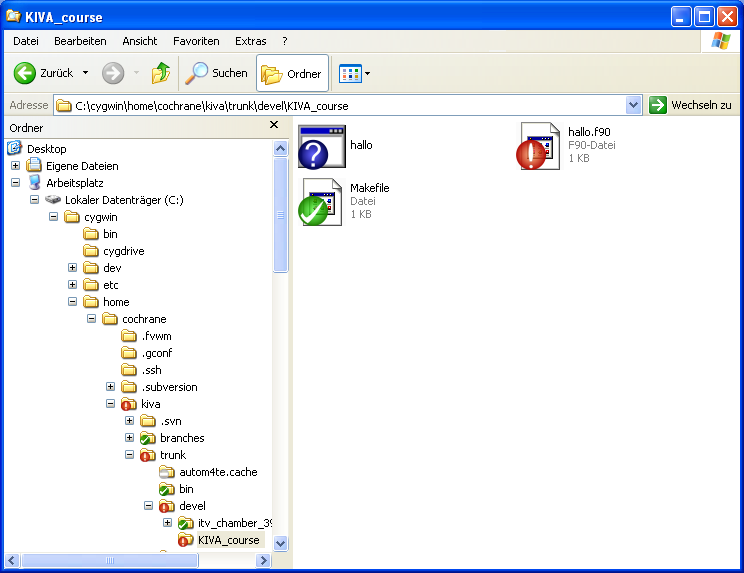
\includegraphics[width=0.5\textwidth]{windows_images/hallo_status_changed.png}
    }
\end{frame}

%%%%%%%%%%%%%%%%%%%%%%%%%%%%%%%%%%%%%%%%%%%%%%%%%%%%%%%%%%%%%%%%%%%%%%%%%%%%
\begin{frame}[fragile]
    \linuxframe
    \frametitle{Let's finally commit something! (cont.)}
    \begin{itemize}
        \item See the differences between the working copy and the cached
            version from the repository
            \begin{itemize}
                \item \ttalert{svn diff} or \ttalert{svn di} or
                    \ttalert{svn di <filename>}
            \end{itemize}
\begin{lstlisting}[basicstyle=\tiny\ttfamily\color{black}]
$ svn diff
Index: hallo.c
===================================================================
--- hallo.c (revision 1)
+++ hallo.c (working copy)
@@ -1,6 +1,6 @@
 #include <stdio.h>
 
 int main(void) {
-    printf("Hallo, Welt!\n");
+    printf("Moin, moin!\n");
     return(0);
 }
\end{lstlisting}
    \begin{itemize}
    \item The output is in \enquote{unified diff} format: \ttalert{diff -u}
    \item A \enquote{unified diff} shows no only what has changed, however
        also (per default) 3 lines of context
    \end{itemize}
\end{itemize}
\end{frame}

%%%%%%%%%%%%%%%%%%%%%%%%%%%%%%%%%%%%%%%%%%%%%%%%%%%%%%%%%%%%%%%%%%%%%%%%%%%%
\begin{frame}[fragile]
    \frametitle{Let's finally commit something! (cont.)}
    \begin{itemize}
        \item See the differences between the working copy and the cached
            version from the repository
            \begin{itemize}
                \item right-click on the changed file; a menu appears
                \item select \ttt{TortoiseSVN} $\rightarrow$ \ttt{Diff}
            \end{itemize}
    \end{itemize}
    \begin{center}
        \begin{tabularx}{\textwidth}{cX}
            %\imagetop{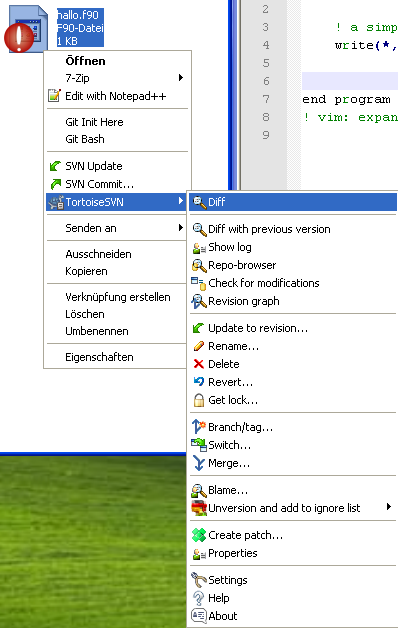
\includegraphics[height=0.5\textheight]{windows_images/hallo_diff_context_menu.png}}
            &
            %\imagetop{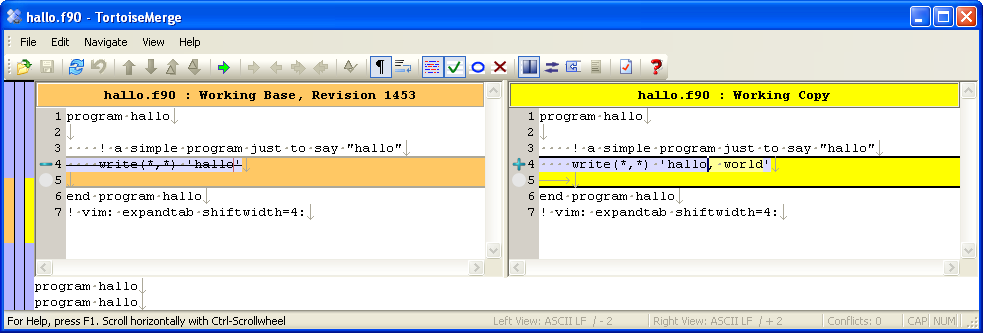
\includegraphics[height=0.35\textheight]{windows_images/hallo_diff_viewer.png}}
        \end{tabularx}
    \end{center}
\end{frame}

%%%%%%%%%%%%%%%%%%%%%%%%%%%%%%%%%%%%%%%%%%%%%%%%%%%%%%%%%%%%%%%%%%%%%%%%%%%%
\begin{frame}[fragile]
    \linuxframe
    \frametitle{Let's finally commit something! (cont.)}
    \begin{itemize}
        \item We know that the program works as we wish:
\begin{lstlisting}
$ ./hallo 
Moin, moin!
\end{lstlisting}
        \item Yay!  Now we can commit our change
        \begin{itemize}
            \item \ttalert{svn commit} or \ttalert{svn ci} or
                \ttalert{svn ci <filename>}
            \item \ttalert{ci} is a short form for \enquote{check in}
        \end{itemize}
\begin{lstlisting}
$ svn commit -m "Using a northern German greeting" hallo.c
Sending        hallo.c
Transmitting file data .
Committed revision 2.
\end{lstlisting}
        \item Our first commit has been checked in!
    \end{itemize}
\end{frame}

%%%%%%%%%%%%%%%%%%%%%%%%%%%%%%%%%%%%%%%%%%%%%%%%%%%%%%%%%%%%%%%%%%%%%%%%%%%%
\begin{frame}[fragile]
    \frametitle{Let's finally commit something! (cont.)}
    \begin{itemize}
        \item We know that the program works as we wish: (Cygwin)
\begin{lstlisting}
$ ./hallo
 hallo, world
\end{lstlisting}
        \item Yay!  Now we can commit our change
        \item Right-click on the file to commit
        \item Select \ttt{SVN Commit...}
    \end{itemize}
    \begin{textblock}{0}(9,-3.5)
        %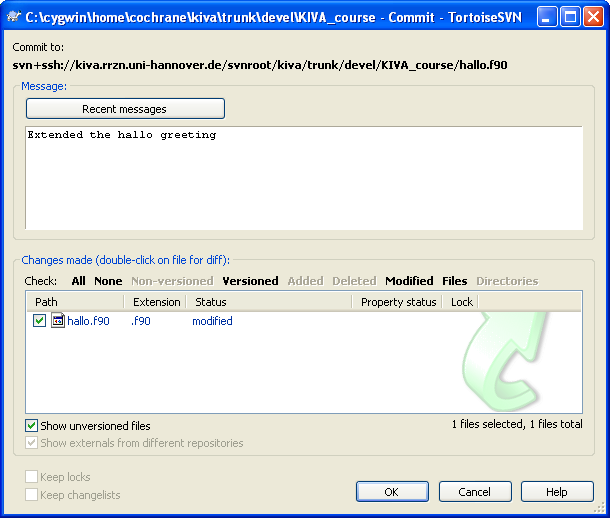
\includegraphics[width=40mm]{windows_images/hallo_commit_window.png}
    \end{textblock}
    \begin{itemize}
        \item Enter the commit message
        \item Click on \ttt{OK}
    \end{itemize}
    \begin{textblock}{0}(9,-0.5)
        %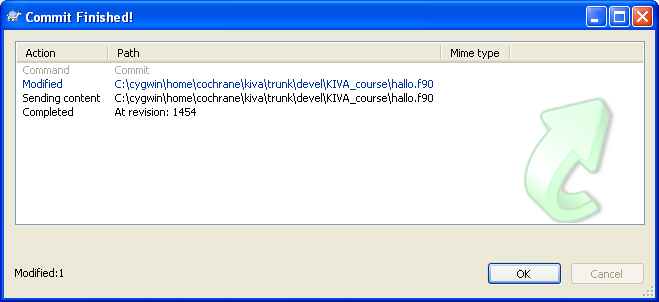
\includegraphics[width=40mm]{windows_images/hallo_commit_progress_window.png}
    \end{textblock}
    \begin{itemize}
        \item Our first commit has been checked in!
    \end{itemize}
\end{frame}

%%%%%%%%%%%%%%%%%%%%%%%%%%%%%%%%%%%%%%%%%%%%%%%%%%%%%%%%%%%%%%%%%%%%%%%%%%%%
\subsection{Workflow}
\begin{frame}{Workflow}
    \linuxframe
    Preparation
    \begin{itemize}
        \item \ttalert{svn import} (only once)
        \item \ttalert{svn checkout/co} (usually only once)
    \end{itemize}

    Main steps
    \begin{itemize}
        \item \ttalert{svn mkdir}
        \item \ttalert{svn move/mv}
        \item \ttalert{svn status/st}
        \item \ttalert{svn diff/di}
        \item \ttalert{svn add} (only once per file)
        \item \ttalert{svn remove/rm}
        \item \ttalert{svn log}
        \item \ttalert{svn update/up}
        \item \ttalert{svn commit/ci}
    \end{itemize}
\end{frame}

%%%%%%%%%%%%%%%%%%%%%%%%%%%%%%%%%%%%%%%%%%%%%%%%%%%%%%%%%%%%%%%%%%%%%%%%%%%%
\begin{frame}{Workflow}
    \windowsframe
    \newlength{\tortoisetab}
    \setlength{\tortoisetab}{50mm}
    Preparation
    \begin{itemize}
        \item Import (only once) \tabto{\tortoisetab}
            \ttt{TortoiseSVN} $\rightarrow$ \ttt{Import...}
        \item Check out \tabto{\tortoisetab}
            \ttt{SVN Checkout...}
    \end{itemize}

    Main steps
    \begin{itemize}
        \item Rename file(s) \tabto{\tortoisetab}
            \ttt{TortoiseSVN} $\rightarrow$ \ttt{Rename...}
        \item See differences \tabto{\tortoisetab}
            \ttt{TortoiseSVN} $\rightarrow$ \ttt{Diff}
        \item Add files (only once per file) \tabto{\tortoisetab}
            \ttt{TortoiseSVN} $\rightarrow$ \ttt{Add}
        \item Delete files \tabto{\tortoisetab}
            \ttt{TortoiseSVN} $\rightarrow$ \ttt{Delete}
        \item See the commit log \tabto{\tortoisetab}
            \ttt{TortoiseSVN} $\rightarrow$ \ttt{Show log}
        \item Update the working copy \tabto{\tortoisetab}
            \ttt{SVN Update}
        \item Commit changes \tabto{\tortoisetab}
            \ttt{SVN Commit...}
    \end{itemize}
\end{frame}

%%%%%%%%%%%%%%%%%%%%%%%%%%%%%%%%%%%%%%%%%%%%%%%%%%%%%%%%%%%%%%%%%%%%%%%%%%%%
\begin{frame}[fragile]
    \linuxframe
    \frametitle{Hallo again}
    Let's play with the \ttalert{hallo} project a bit more.  However this
    time we'll work on it together.

    Check out the project: \ttalert{svn checkout}/\ttalert{svn co}
\begin{lstlisting}
$ svn co svn+ssh://vcskurs15@host.name/svnroot/projects/hallo\
     hallo_gemeinsam
A    hallo_gemeinsam/hallo.c
A    hallo_gemeinsam/Makefile
Checked out revision 1.
\end{lstlisting}

The standard Subversion directory structure doesn't yet exist in this case.
One of us can create these directories:
\begin{lstlisting}
$ svn mkdir trunk branches tags
A         trunk
A         branches
A         tags
\end{lstlisting}
\end{frame}

%%%%%%%%%%%%%%%%%%%%%%%%%%%%%%%%%%%%%%%%%%%%%%%%%%%%%%%%%%%%%%%%%%%%%%%%%%%%
\begin{frame}[fragile]
    \frametitle{Hallo again (cont.)}
    \linuxframe
    Show the status of the working copy:
\begin{lstlisting}
$ svn status
A      trunk
A      branches
A      tags
\end{lstlisting}

Now we can move the files into the \ttalert{trunk} directory:
\begin{lstlisting}
$ svn mv hallo.c trunk/
A         trunk/hallo.c
D         hallo.c
$ svn mv Makefile trunk/
A         trunk/Makefile
D         Makefile
\end{lstlisting}

\end{frame}

%%%%%%%%%%%%%%%%%%%%%%%%%%%%%%%%%%%%%%%%%%%%%%%%%%%%%%%%%%%%%%%%%%%%%%%%%%%%
\begin{frame}[fragile]
    \frametitle{Hallo again (cont.)}
    \linuxframe
    The status in the working copy is now more interesting:
\begin{lstlisting}
$ svn st
D      hallo.c
A      trunk
A  +   trunk/hallo.c
A  +   trunk/Makefile
A      branches
D      Makefile
A      tags
\end{lstlisting}

    Points of note:
    \begin{itemize}
        \item Creating directories is a process in Subversion, not only from the OS
        \item A \enquote{move} of a file creates the file first at the new location
            and then deletes the old location
        \item The history of a file or directory comes with the file to its new
            location.  This was a huge improvement over CVS.
    \end{itemize}
\end{frame}

%%%%%%%%%%%%%%%%%%%%%%%%%%%%%%%%%%%%%%%%%%%%%%%%%%%%%%%%%%%%%%%%%%%%%%%%%%%%
\begin{frame}[fragile]
    \frametitle{Hallo again (cont.)}
    \linuxframe
    The changes can be checked in:
\begin{lstlisting}
$ svn ci
Deleting       Makefile
Adding         branches
Deleting       hallo.c
Adding         tags
Adding         trunk
Adding         trunk/Makefile
Adding         trunk/hallo.c

Committed revision 2.
\end{lstlisting}
\end{frame}

%%%%%%%%%%%%%%%%%%%%%%%%%%%%%%%%%%%%%%%%%%%%%%%%%%%%%%%%%%%%%%%%%%%%%%%%%%%%
\begin{frame}[fragile]
    \frametitle{Hallo again (cont.)}
    \linuxframe

    Now everyone can update their working copy to the latest version:
    \ttalert{svn update}/\ttalert{svn up}.

    \begin{lstlisting}[basicstyle=\tiny\ttfamily\color{black}]
$ svn up
D    hallo.c
D    Makefile
A    trunk
A    trunk/hallo.c
A    trunk/Makefile
A    branches
A    tags
Updated to revision 2.
\end{lstlisting}

    Again Subversion shows us what it's doing:
    \begin{itemize}
        \item The \ttalert{hallo.c} and \ttalert{Makefile} files were
            deleted from the current directory (\ttalert{D})
        \item The \ttalert{trunk}, \ttalert{branches} and \ttalert{tags}
            directories were created (added) (\ttalert{A})
        \item And the \ttalert{hallo.c} and \ttalert{Makefile} files were
            added to the \ttalert{trunk} directory (\ttalert{A}).
    \end{itemize}
\end{frame}

%%%%%%%%%%%%%%%%%%%%%%%%%%%%%%%%%%%%%%%%%%%%%%%%%%%%%%%%%%%%%%%%%%%%%%%%%%%%
\begin{frame}[fragile]
    \frametitle{Hallo again (cont.)}
    \linuxframe

We want to have a list of things that we want to add to the \ttalert{hallo}
project.  Therefore we create a file called \ttalert{TODO}:
\begin{lstlisting}
$ cd trunk/
$ echo "# TODO list for the hallo project" > TODO
$ svn status
?      TODO
\end{lstlisting}

Subversion doesn't yet know about this file.  This is why a question mark
shows up in the first (left-most) column.

In order that Subversion knows about the new file, we need to \emph{add} the
file:
\begin{lstlisting}
$ svn add TODO
A         TODO
\end{lstlisting}
\end{frame}

%%%%%%%%%%%%%%%%%%%%%%%%%%%%%%%%%%%%%%%%%%%%%%%%%%%%%%%%%%%%%%%%%%%%%%%%%%%%
\begin{frame}[fragile]
    \frametitle{Hallo again (cont.)}
    \linuxframe

    The addition of the file to Subversion is also a \emph{change},
    therefore we need to check in (commit) this:
\begin{lstlisting}[basicstyle=\tiny\ttfamily\color{black}]
$ svn ci -m "Added a TODO list" TODO 
Adding         TODO
Transmitting file data .
Committed revision 3.
\end{lstlisting}

Now we can add ideas to our TODO list:
\begin{lstlisting}[basicstyle=\tiny\ttfamily\color{black}]
$ cat TODO
# TODO list for the hallo project
 - hallo in different languages
 - say "hallo" many times
\end{lstlisting}

Now look at the status
\begin{lstlisting}[basicstyle=\tiny\ttfamily\color{black}]
$ svn st
M      TODO
\end{lstlisting}
The file has been changed, which is why a \ttalert{M} appears in the first
column.
\end{frame}

%%%%%%%%%%%%%%%%%%%%%%%%%%%%%%%%%%%%%%%%%%%%%%%%%%%%%%%%%%%%%%%%%%%%%%%%%%%%
\begin{frame}[fragile]
    \frametitle{Hallo again (cont.)}
    \linuxframe

Looking at the diffs helps to make sure that what one is about to commit, is
exactly that which one wants to commit.
\begin{lstlisting}[basicstyle=\tiny\ttfamily\color{black}]
$ svn di
Index: TODO
===================================================================
--- TODO    (revision 3)
+++ TODO    (working copy)
@@ -1 +1,3 @@
 # TODO list for the hallo project
+ - hallo in different languages
+ - say "hallo" many times
\end{lstlisting}

And as per usual, we push this information in a commit to the server:
\begin{lstlisting}[basicstyle=\tiny\ttfamily\color{black}]
svn ci -m "Wrote a few ideas for the hallo project"
Sending        trunk/TODO
Transmitting file data .
Committed revision 4.
\end{lstlisting}

\end{frame}

%%%%%%%%%%%%%%%%%%%%%%%%%%%%%%%%%%%%%%%%%%%%%%%%%%%%%%%%%%%%%%%%%%%%%%%%%%%%
\begin{frame}[fragile]
    \frametitle{Hallo again}
    Let's play with the \ttalert{hallo} project a bit more.  However this
    time we'll work on it together.

    We want to have a list of things that we want to add to the \ttalert{hallo}
    project.  Therefore we create a file called \ttalert{TODO} with \notepad:

    \begin{center}
        %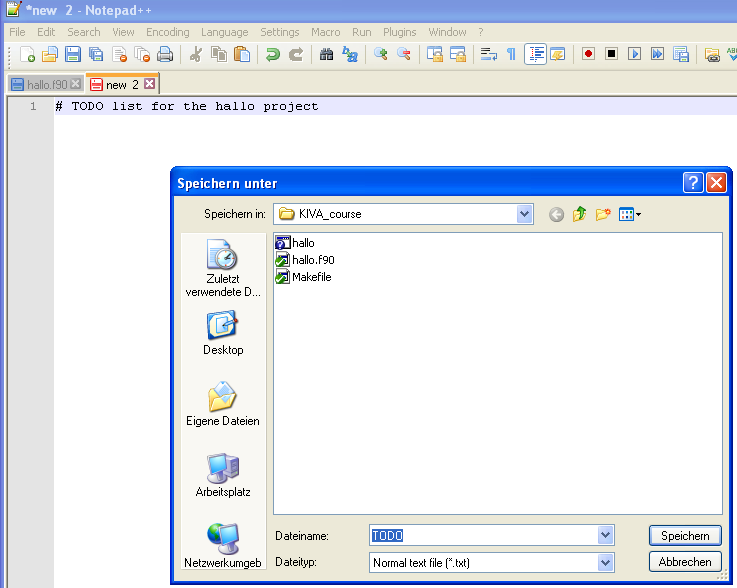
\includegraphics[width=0.5\textwidth]{windows_images/notepadpp_new_todo.png}
    \end{center}
\end{frame}

%%%%%%%%%%%%%%%%%%%%%%%%%%%%%%%%%%%%%%%%%%%%%%%%%%%%%%%%%%%%%%%%%%%%%%%%%%%%
\begin{frame}[fragile]
    \frametitle{Hallo again}
    Subversion doesn't yet know about this file.  This is why a blue
    question mark appears on the file's icon.

    \begin{center}
        %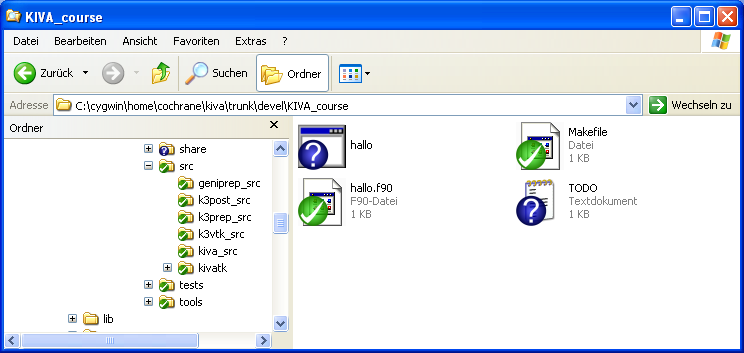
\includegraphics[width=0.7\textwidth]{windows_images/todo_file_unknown.png}
    \end{center}
\end{frame}

%%%%%%%%%%%%%%%%%%%%%%%%%%%%%%%%%%%%%%%%%%%%%%%%%%%%%%%%%%%%%%%%%%%%%%%%%%%%
\begin{frame}[fragile]
    \frametitle{Hallo again}

    In order that Subversion knows about the new file, we need to \emph{add} the
    file.
    \begin{itemize}
        \item right-click on the file
        \item \ttt{Tortoise SVN} $\rightarrow$ \ttt{Add}
        \item a blue plus-sign shows up on the file just added
    \end{itemize}

    \begin{center}
        \begin{tabularx}{\textwidth}{cX}
            %\imagetop{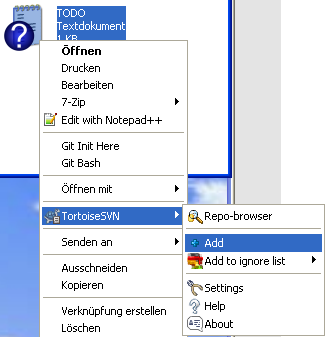
\includegraphics[width=0.3\textwidth]{windows_images/add_todo_file.png}}
            &
            %\imagetop{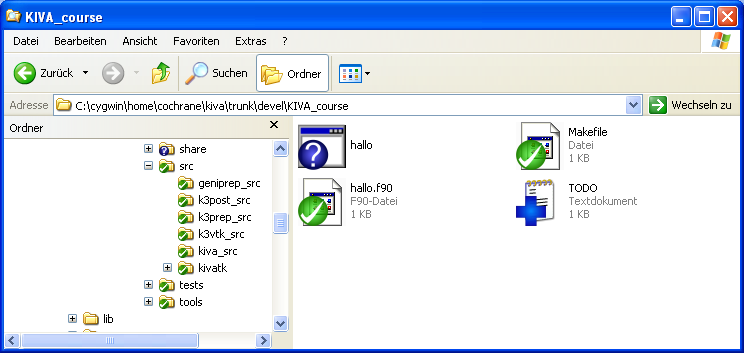
\includegraphics[width=0.6\textwidth]{windows_images/todo_file_added.png}}
        \end{tabularx}
    \end{center}
\end{frame}

%%%%%%%%%%%%%%%%%%%%%%%%%%%%%%%%%%%%%%%%%%%%%%%%%%%%%%%%%%%%%%%%%%%%%%%%%%%%
\begin{frame}[fragile]
    \frametitle{Hallo again (cont.)}

    The addition of the file to Subversion is also a \emph{change},
    therefore we need to check in (commit) this:
    \begin{itemize}
        \item right-click in the directory containing the new TODO file
            \begin{itemize}
                \item it isn't necessary to commit files individually
                \item Subversion performs commits recursively from the
                    directory where the commit is started
            \end{itemize}
        \item select \ttt{SVN Commit...}
    \end{itemize}

    \begin{textblock}{0}(7,-1.5)
        %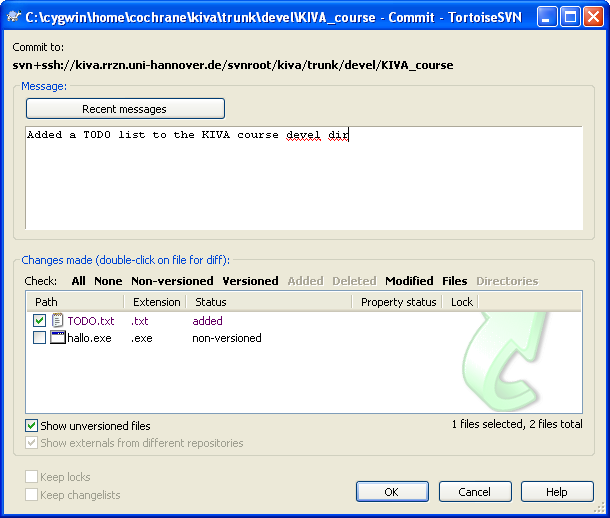
\includegraphics[width=50mm]{windows_images/commit_todo_file.png}
    \end{textblock}

    \begin{itemize}
        \item add a commit message
        \item click on \ttt{OK}
    \end{itemize}
\end{frame}

%%%%%%%%%%%%%%%%%%%%%%%%%%%%%%%%%%%%%%%%%%%%%%%%%%%%%%%%%%%%%%%%%%%%%%%%%%%%
\begin{frame}[fragile]
    \frametitle{Hallo again (cont.)}

    \begin{itemize}
        \item Now we can add ideas to our TODO list:
    \end{itemize}
    \begin{center}
        %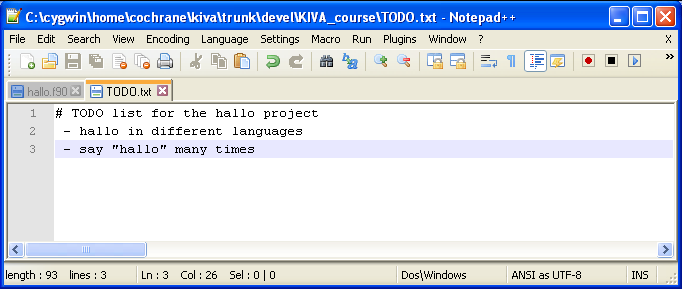
\includegraphics[width=0.45\textwidth]{windows_images/todo_file_more_items.png}
    \end{center}

    \begin{itemize}
        \item The TODO file has a red exclamation mark: its contents have changed.
    \end{itemize}
    \begin{center}
        %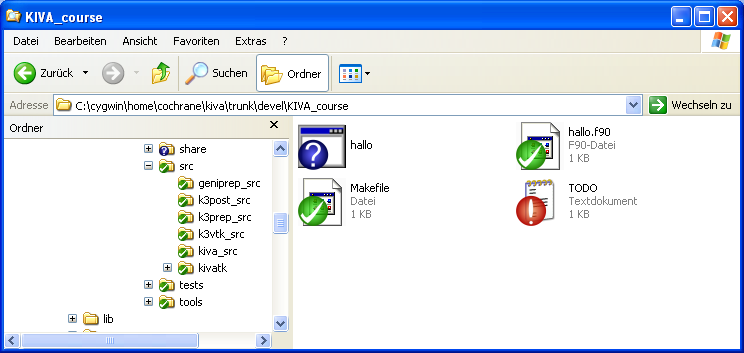
\includegraphics[width=0.45\textwidth]{windows_images/todo_file_changed.png}
    \end{center}
\end{frame}

%%%%%%%%%%%%%%%%%%%%%%%%%%%%%%%%%%%%%%%%%%%%%%%%%%%%%%%%%%%%%%%%%%%%%%%%%%%%
\begin{frame}[fragile]
    \frametitle{Hallo again (cont.)}

    Looking at the diffs helps to make sure that what one is about to commit, is
    exactly that which one wants to commit.
    \begin{itemize}
        \item right-click on the TODO icon
        \item \ttt{Tortoise SVN} $\rightarrow$ \ttt{Diff}
    \end{itemize}
    \begin{center}
        %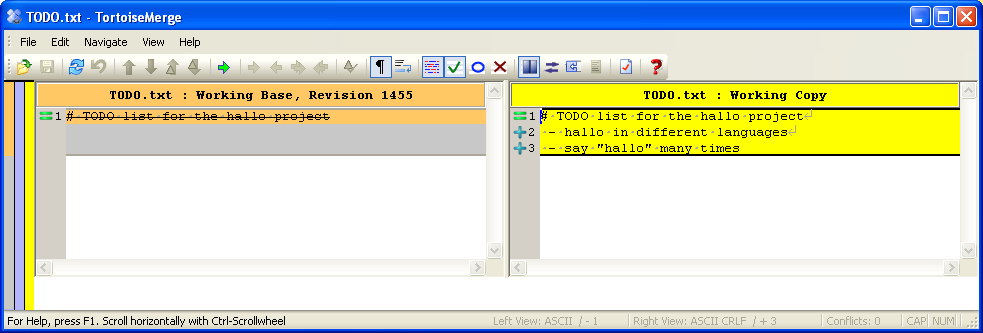
\includegraphics[width=0.8\textwidth]{windows_images/todo_file_diff.png}
    \end{center}

\end{frame}

%%%%%%%%%%%%%%%%%%%%%%%%%%%%%%%%%%%%%%%%%%%%%%%%%%%%%%%%%%%%%%%%%%%%%%%%%%%%
\begin{frame}[fragile]
    \frametitle{Hallo again (cont.)}

    And as per usual, we push this information in a commit to the server:
    \begin{itemize}
        \item right-click on the TODO icon or simply somewhere in the
            directory
        \item \ttt{SVN Commit...}
        \item enter a commit message
        \item click on \ttt{OK}
    \end{itemize}
    \begin{center}
        %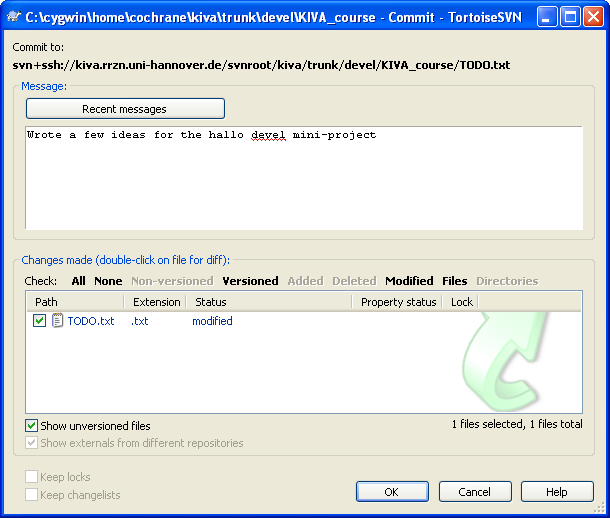
\includegraphics[width=0.4\textwidth]{windows_images/todo_file_commit_new_changes.png}
    \end{center}

\end{frame}

%%%%%%%%%%%%%%%%%%%%%%%%%%%%%%%%%%%%%%%%%%%%%%%%%%%%%%%%%%%%%%%%%%%%%%%%%%%%
\begin{frame}[fragile]
    \frametitle{Hallo again (cont.)}

    The versioned files in the directory are again all green, and our
    working copy is again \enquote{clean}.
    \begin{center}
        %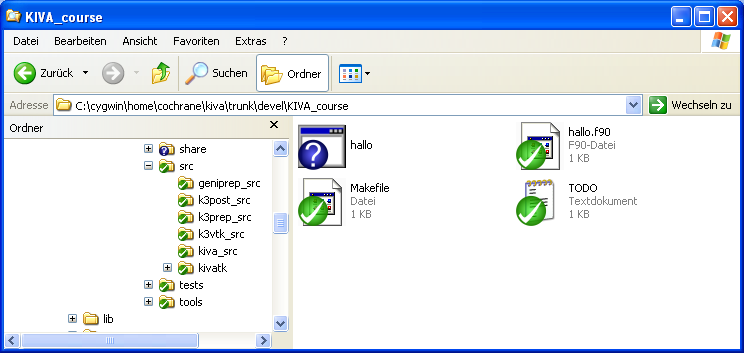
\includegraphics[width=0.6\textwidth]{windows_images/clean_working_dir.png}
    \end{center}

\end{frame}

%%%%%%%%%%%%%%%%%%%%%%%%%%%%%%%%%%%%%%%%%%%%%%%%%%%%%%%%%%%%%%%%%%%%%%%%%%%%
\begin{frame}[fragile]
    \frametitle{Hallo again (cont.)}

    Now \emph{you} can update your working copies to the current repository
    status:
    \begin{itemize}
        \item right-click in the \ttt{vcs\_course} directory
        \item select \ttt{SVN Update}
        \item you should see your working copy be updated
        \item you should now see the \ttt{TODO} file
    \end{itemize}
    \begin{center}
        %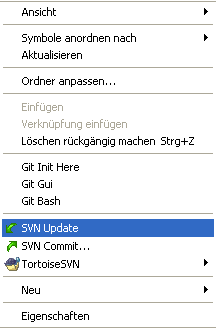
\includegraphics[width=0.2\textwidth]{windows_images/update_working_dir.png}
    \end{center}

\end{frame}

%%%%%%%%%%%%%%%%%%%%%%%%%%%%%%%%%%%%%%%%%%%%%%%%%%%%%%%%%%%%%%%%%%%%%%%%%%%%
\begin{frame}[fragile]
    \frametitle{Exercise---develop \ttalert{hallo} further}

    Each course member should do the following (one after the other):
    \begin{itemize}
        \item update the working directory
        \item add another \enquote{hallo} to the \ttalert{hallo.f90} file
        \item build the mini-project with \ttalert{make}
        \item view the diff
        \item commit the result with a good commit message
    \end{itemize}
\end{frame}

%%%%%%%%%%%%%%%%%%%%%%%%%%%%%%%%%%%%%%%%%%%%%%%%%%%%%%%%%%%%%%%%%%%%%%%%%%%%
\begin{frame}[fragile]
    \frametitle{Seeing what we've done}
    \linuxframe

    In order to see what has been done in the past, one uses usually a
    cobination of \ttalert{svn log} (coarse-grained information) and
    \ttalert{svn diff} (detailed information).

\begin{lstlisting}[basicstyle=\tiny\ttfamily\color{black}]
$ svn log
------------------------------------------------------------------------
r3 | vcskurs15 | 2010-09-15 19:00:43 +0200 (Wed, 15 Sep 2010) | 1 line

Added a TODO list
------------------------------------------------------------------------
r2 | vcskurs15 | 2010-09-15 18:24:12 +0200 (Wed, 15 Sep 2010) | 3 lines

Created the standard Subversion directory structure and moved the files into trunk
------------------------------------------------------------------------
\end{lstlisting}

Sometimes not all commits which have been checked are shown.  This happens
because the working copy isn't up to date with the server.  Running 
\ttalert{svn update} corrects this.
\end{frame}

%%%%%%%%%%%%%%%%%%%%%%%%%%%%%%%%%%%%%%%%%%%%%%%%%%%%%%%%%%%%%%%%%%%%%%%%%%%%
\begin{frame}[fragile]
    \frametitle{Seeing what we've done (cont.)}
    \linuxframe
    \vspace*{-3mm}
\begin{lstlisting}[basicstyle=\tiny\ttfamily\color{black}]
$ svn log --verbose
------------------------------------------------------------------------
r5 | vcskurs15 | 2010-09-17 10:27:30 +0200 (Fri, 17 Sep 2010) | 2 lines
Changed paths:
   M /trunk/TODO
   M /trunk/hallo.c
Added new languages
------------------------------------------------------------------------
r4 | vcskurs15 | 2010-09-15 19:22:59 +0200 (Wed, 15 Sep 2010) | 1 line
Changed paths:
   M /trunk/TODO
Wrote a few ideas for the hallo project
------------------------------------------------------------------------
r3 | vcskurs15 | 2010-09-15 19:00:43 +0200 (Wed, 15 Sep 2010) | 1 line
Changed paths:
   A /trunk/TODO
Added a TODO list
------------------------------------------------------------------------
r2 | vcskurs15 | 2010-09-15 18:24:12 +0200 (Wed, 15 Sep 2010) | 3 lines
Changed paths:
   D /Makefile
   A /branches
   D /hallo.c
   A /tags
   A /trunk
   A /trunk/Makefile (from /Makefile:1)
   A /trunk/hallo.c (from /hallo.c:1)
Created the standard Subversion directory structure and moved the files into trunk
------------------------------------------------------------------------
\end{lstlisting}
\end{frame}

%%%%%%%%%%%%%%%%%%%%%%%%%%%%%%%%%%%%%%%%%%%%%%%%%%%%%%%%%%%%%%%%%%%%%%%%%%%%
\begin{frame}[fragile]
    \frametitle{Seeing what we've done (cont.)}
    \linuxframe
    \vspace*{-2mm}
    Show the difference between the working copy and the \ttalert{HEAD} revision.
\begin{lstlisting}
$ svn diff [<filename>]
\end{lstlisting}

\begin{lstlisting}[basicstyle=\tiny\ttfamily\color{black}]
$ svn diff hallo.c
Index: hallo.c
===================================================================
--- hallo.c (revision 3)
+++ hallo.c (working copy)
@@ -1,6 +1,17 @@
+// hallo: a program to say "hallo!"
 #include <stdio.h>
 
 int main(void) {
+    // north
     printf("Moin, moin!\n");
+    // middle
+    printf("Tach!\n");
+    printf("Halli hallo!\n");
+    // south
+    printf("Gruess Gott!\n");
+    // further south
+    printf("Gruetzi!\n");
+    // even further south...
+    printf("Gudday!\n");
     return(0);
 }
\end{lstlisting}
\end{frame}

%%%%%%%%%%%%%%%%%%%%%%%%%%%%%%%%%%%%%%%%%%%%%%%%%%%%%%%%%%%%%%%%%%%%%%%%%%%%
\begin{frame}[fragile]
    \frametitle{Seeing what we've done (cont.)}
    \linuxframe
    \vspace*{-2mm}
    Show the difference between different revisions
\begin{lstlisting}
$ svn diff -r M:N [<filename>]
\end{lstlisting}

\begin{lstlisting}[basicstyle=\tiny\ttfamily\color{black}]
$ svn di -r2:5 hallo.c
Index: hallo.c
===================================================================
--- hallo.c (revision 2)
+++ hallo.c (revision 5)
@@ -1,6 +1,17 @@
+// hallo: a program to say "hallo"!
 #include <stdio.h>
 
 int main(void) {
+    // north
     printf("Moin, moin!\n");
+    // middle
+    printf("Tach!\n");
+    printf("Halli hallo!\n");
+    // south
+    printf("Gruess Gott!\n");
+    // further south
+    printf("Gruetzi!\n");
+    // even further south...
+    printf("Gudday!\n");
     return(0);
 }
\end{lstlisting}

\end{frame}

%%%%%%%%%%%%%%%%%%%%%%%%%%%%%%%%%%%%%%%%%%%%%%%%%%%%%%%%%%%%%%%%%%%%%%%%%%%%
\begin{frame}[fragile]
    \frametitle{Seeing what we've done (cont.)}
    \linuxframe
    \vspace*{-2mm}
    Show the differences in the last \emph{change}
\begin{lstlisting}
$ svn diff -c N [<filename>]
\end{lstlisting}

\begin{lstlisting}
$ svn di -c 4
Index: TODO
===================================================================
--- TODO    (revision 3)
+++ TODO    (revision 4)
@@ -1 +1,3 @@
 # TODO list for the hallo project
+ - hallo in different languages
+ - say "hallo" many times
\end{lstlisting}

\end{frame}

%%%%%%%%%%%%%%%%%%%%%%%%%%%%%%%%%%%%%%%%%%%%%%%%%%%%%%%%%%%%%%%%%%%%%%%%%%%%
\subsection{Fixing errors}

\begin{frame}[fragile]
    \frametitle{When errors occur\ldots}
    There are many things which can happen daily which aren't necessarily
    wished for.
    \begin{itemize}
        \item one deletes a file by mistake
        \item one makes changes which are no longer relevant
        \item one makes a commit which contained an error
    \end{itemize}
    With version control it's possible to solve such problems very easily.

    In Subversion one solves such problems like so:
\end{frame}

%%%%%%%%%%%%%%%%%%%%%%%%%%%%%%%%%%%%%%%%%%%%%%%%%%%%%%%%%%%%%%%%%%%%%%%%%%%%
\begin{frame}[fragile]
    \frametitle{When errors occur\ldots (cont.)}
    \linuxframe
    \vspace*{-3mm}
    \begin{alertblock}{The mistakenly deleted file}
        The solutions: \ttalert{svn update} or \ttalert{svn revert}

        An \ttalert{update} retrieves the current version of the file from
        the \ttalert{HEAD} revision on the server.
\begin{lstlisting}[basicstyle=\tiny\ttfamily\color{black}]
$ rm hallo.c   # oops!
$ svn up       # this would work with 'svn revert' as well
Restored 'hallo.c'
At revision 6.
$ ls           # it's there again!
hallo.c  Makefile
\end{lstlisting}

    Or a little bit worse, if one had used Subversion to delete the file:
\begin{lstlisting}[basicstyle=\tiny\ttfamily\color{black}]
$ svn rm hallo.c   # oops!
D         hallo.c
$ svn revert hallo.c
Restored 'hallo.c'
At revision 6.
$ ls               # it's there again!
hallo.c  Makefile
\end{lstlisting}
    \end{alertblock}

\end{frame}

%%%%%%%%%%%%%%%%%%%%%%%%%%%%%%%%%%%%%%%%%%%%%%%%%%%%%%%%%%%%%%%%%%%%%%%%%%%%
\begin{frame}[fragile]
    \frametitle{When errors occur\ldots (cont.)}
    \linuxframe
    \vspace*{-3mm}
    \begin{alertblock}{Irrelevant code changes}
        Let's say that we make an unwanted change.
\begin{lstlisting}[basicstyle=\tiny\ttfamily\color{black}]
$ svn di
Index: hallo.c
===================================================================
--- hallo.c (revision 6)
+++ hallo.c (working copy)
@@ -13,5 +13,7 @@
     printf("Gruetzi!\n");
     // even further south...
     printf("Gudday!\n");
+    // still further south
+    printf("Arf!  Arf!  Arf!\n");
     return(0);
 }
\end{lstlisting}
    One notices that this is getting silly and wants to \enquote{undo} this
    change.
    %Dieses Beispiel ist doch etwas kurz, aber stellt euch
    %vor, dass man mehere Dateien geändert hat und mehere Zeilen in jeder Datei.
    The solution: \ttalert{svn revert}
\begin{lstlisting}[basicstyle=\tiny\ttfamily\color{black}]
$ svn revert hallo.c
Reverted 'hallo.c'
\end{lstlisting}

\end{alertblock}
\end{frame}

%%%%%%%%%%%%%%%%%%%%%%%%%%%%%%%%%%%%%%%%%%%%%%%%%%%%%%%%%%%%%%%%%%%%%%%%%%%%
\begin{frame}[fragile]
    \frametitle{When errors occur\ldots (cont.)}
    \linuxframe
    \begin{alertblock}{The erroneous commit}
        We find out at some point in the development, that the commit in
        revision \ttalert{<x>} was wrong and we want undo this change.

        The solution: one does a \enquote{rollback}.

        There are several ways to do a \enquote{rollback}:
        \begin{itemize}
            \item \ttalert{svn up -r N}; \ttalert{cp file file.fixed};
                \ttalert{svn up};\\
                \ttalert{cp file.fixed file}; \ttalert{svn ci}
            \item \ttalert{svn di -r NEW:OLD > change.patch};\\
                \ttalert{patch -p0 < change.patch}; \ttalert{svn ci}
            \item \ttalert{svn merge -r NEW:OLD <URL>} or
                \ttalert{svn merge -c -NEW <URL>}; then
                \ttalert{svn ci}.  This works with Subversion Version 1.5+.
                See also \hyperlink{branch-merge}{\alert{Branching and
                Merging}} later.
        \end{itemize}
    \end{alertblock}
\end{frame}

%%%%%%%%%%%%%%%%%%%%%%%%%%%%%%%%%%%%%%%%%%%%%%%%%%%%%%%%%%%%%%%%%%%%%%%%%%%%
\begin{frame}[fragile]
\frametitle{Rollback with \ttalert{svn diff}}
\linuxframe

\begin{center}
    \resizebox{\textwidth}{!}{
        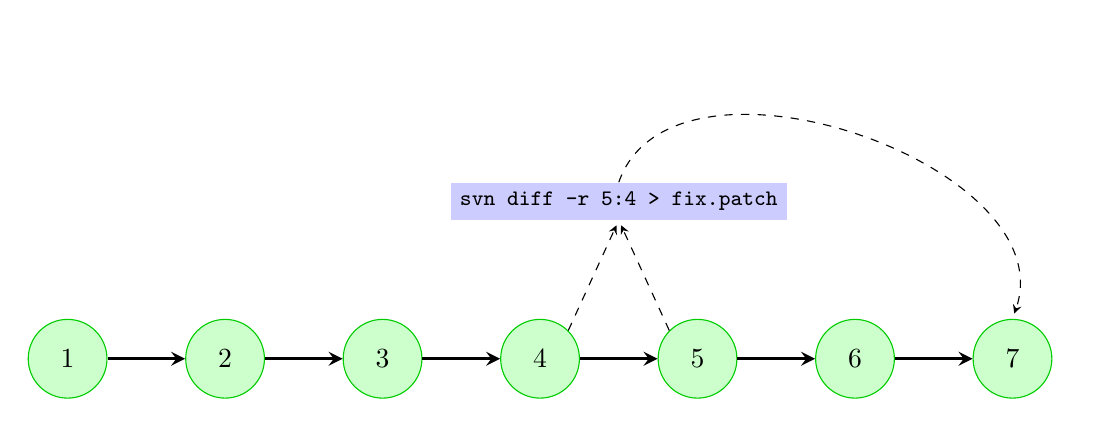
\begin{tikzpicture}
[rev/.style = {circle,
		draw=green!80!black,
		minimum size=10mm,
		fill=green!20!white},
 op/.style  = {fill=blue!20},
 trans/.style = {->,very thick,>=stealth}]
% line of development
\node[rev] at (0,0) (rev1) [] {1};
\node[rev] at (2,0) (rev2) [] {2};
\draw [trans] (rev1.east) -- (rev2.west);
\node[rev] at (4,0) (rev3) [] {3};
\draw [trans] (rev2.east) -- (rev3.west);
\node[rev] at (6,0) (rev4) [] {4};
\draw [trans] (rev3.east) -- (rev4.west);
\node[rev] at (8,0) (rev5) [] {5};
\draw [trans] (rev4.east) -- (rev5.west);
\node[rev] at (10,0) (rev6) [] {6};
\draw [trans] (rev5.east) -- (rev6.west);
% diff between revisions 4 and 5
\node[op] at (7, 2) (diff) {\footnotesize\texttt{svn diff -r 5:4 > fix.patch}};
\draw [->,>=stealth,dashed,shorten >=2pt] (rev4.north east) -- (diff.south);
\draw [->,>=stealth,dashed,shorten >=2pt] (rev5.north west) -- (diff.south);
% revision 7
\node[rev] at (12,0) (rev7) [] {7};
\draw [trans] (rev6.east) -- (rev7.west);
% fast forward to revision 7
\draw [->,>=stealth,dashed,shorten >=2pt,bend left=90] (diff.north) to (rev7.north);
\end{tikzpicture}

    }
\end{center}

\begin{lstlisting}
$ svn diff -r 5:4 > fix.patch
$ patch -p0 < fix.patch
$ svn ci
Committed revision 7.
\end{lstlisting}

\end{frame}

%%%%%%%%%%%%%%%%%%%%%%%%%%%%%%%%%%%%%%%%%%%%%%%%%%%%%%%%%%%%%%%%%%%%%%%%%%%%
\begin{frame}[fragile]
\frametitle{Rollback with \ttalert{svn merge}}
\linuxframe

\begin{center}
    \resizebox{\textwidth}{!}{
        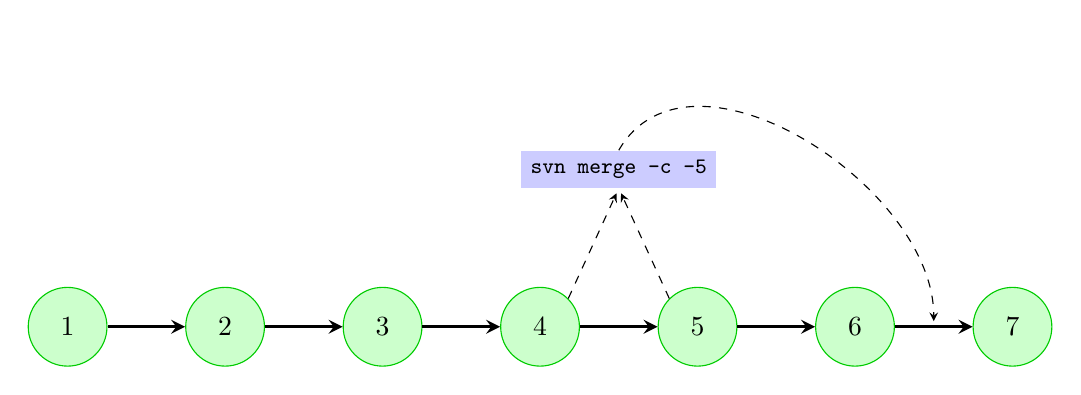
\begin{tikzpicture}
[rev/.style = {circle,
		draw=green!80!black,
		minimum size=10mm,
		fill=green!20!white},
 op/.style  = {fill=blue!20},
 trans/.style = {->,very thick,>=stealth}]
% line of development
\node[rev] at (0,0) (rev1) [] {1};
\node[rev] at (2,0) (rev2) [] {2};
\draw [trans] (rev1.east) -- (rev2.west);
\node[rev] at (4,0) (rev3) [] {3};
\draw [trans] (rev2.east) -- (rev3.west);
\node[rev] at (6,0) (rev4) [] {4};
\draw [trans] (rev3.east) -- (rev4.west);
\node[rev] at (8,0) (rev5) [] {5};
\draw [trans] (rev4.east) -- (rev5.west);
\node[rev] at (10,0) (rev6) [] {6};
\draw [trans] (rev5.east) -- (rev6.west);
% merge from change 5 into commit to revision 7
\node[op] at (7, 2) (merge) {\footnotesize\texttt{svn merge -c -5}};
\draw [->,>=stealth,dashed,shorten >=2pt] (rev4.north east) -- (merge.south);
\draw [->,>=stealth,dashed,shorten >=2pt] (rev5.north west) -- (merge.south);
% revision 7
\node[rev] at (12,0) (rev7) [] {7};
\draw [trans] (rev6.east) -- (rev7.west);
% merge between commits 6 and 7
\draw [->,>=stealth,dashed,shorten >=2pt,out=60,in=90] (merge.north) to (11,0);
\end{tikzpicture}

    }
\end{center}

\begin{lstlisting}
$ svn merge -c -5
$ svn ci
Committed revision 7.
\end{lstlisting}

\end{frame}

%%%%%%%%%%%%%%%%%%%%%%%%%%%%%%%%%%%%%%%%%%%%%%%%%%%%%%%%%%%%%%%%%%%%%%%%%%%%
\begin{frame}[fragile]
    \frametitle{Conflicts}
        When one works with others it is possible that one edits the same
        part of a document as someone else.  When both of these changes are
        checked in they can't be merged automatically: one of them will be
        \emph{in conflict} with the other.  This is a disadvantage of the
        simultaneous editing model, however the advantages are most
        certainly in the majority.

        In order to resovle conflicts one needs a human (since the computer
        can't do it itself) and one needs communication between the humans.
        Subversion also gives some help in solving conflicts: the
        conflicting parts of the document are marked and one can use the
        \ttalert{svn resolved} command to mark conflicts as being corrected.

        Let's try and create a conflict within the \ttalert{hallo} project.

        We have to working copies, \ttalert{hallo1} and \ttalert{hallo2}.
\end{frame}

%%%%%%%%%%%%%%%%%%%%%%%%%%%%%%%%%%%%%%%%%%%%%%%%%%%%%%%%%%%%%%%%%%%%%%%%%%%%
\begin{frame}[fragile]
    \frametitle{Conflicts (cont.)}
    \linuxframe
        Are the working copies up to date?
\begin{lstlisting}[basicstyle=\tiny\ttfamily\color{black}]
$ cd hallo1
$ svn up
U    trunk/hallo.c
U    trunk/TODO
Updated to revision 6.
$ cd ../hallo2
$ svn up
At revision 6.
\end{lstlisting}

Let's change a line in \ttalert{hallo.c} in \ttalert{hallo2}:
\begin{lstlisting}[basicstyle=\tiny\ttfamily\color{black}]
$ svn di hallo.c
Index: hallo.c
===================================================================
--- hallo.c (revision 6)
+++ hallo.c (working copy)
@@ -12,6 +12,6 @@
     // further south
     printf("Gruetzi!\n");
     // even further south...
-    printf("Gudday!\n");
+    printf("Gudday, mate!\n");
     return(0);
 }
\end{lstlisting}
\end{frame}

%%%%%%%%%%%%%%%%%%%%%%%%%%%%%%%%%%%%%%%%%%%%%%%%%%%%%%%%%%%%%%%%%%%%%%%%%%%%
\begin{frame}[fragile]
    \frametitle{Conflicts (cont.)}
    \linuxframe

    The we commit the change:
\begin{lstlisting}
$ svn ci -m "A greeting is a bit more kiwi" hallo.c
Sending        hallo.c
Transmitting file data .
Committed revision 7.
\end{lstlisting}

Now we change the same line in \ttalert{hallo1}:
\begin{lstlisting}[basicstyle=\tiny\ttfamily\color{black}]
$ svn di
Index: hallo.c
===================================================================
--- hallo.c (revision 6)
+++ hallo.c (working copy)
@@ -12,6 +12,6 @@
     // further south
     printf("Gruetzi!\n");
     // even further...
-    printf("Gudday!\n");
+    printf("G'day, mate!\n");
     return(0);
 }
\end{lstlisting}
\end{frame}

%%%%%%%%%%%%%%%%%%%%%%%%%%%%%%%%%%%%%%%%%%%%%%%%%%%%%%%%%%%%%%%%%%%%%%%%%%%%
\begin{frame}[fragile]
    \frametitle{Conflicts (cont.)}
    \linuxframe

But that won't work!  The change in the working copy is with respect to
revision 6 and the current revision in the repository is already at 7.
\emph{Also} the same line was changed!

Exactly!

That's why one should often run \ttalert{svn update} when one works,
especially before one checks something in.  However, this won't help in this
case:

\begin{lstlisting}[basicstyle=\tiny\ttfamily\color{black}]
$ svn up
Conflict discovered in 'hallo.c'.
Select: (p) postpone, (df) diff-full, (e) edit,
        (h) help for more options: 
\end{lstlisting}

What can we do?
    \begin{itemize}
        \item edit the file now
        \item resovle the conflict later
        \item use the revision of the other person
        \item use your own revision
        \item look at the \ttalert{diff} and then decide what to do
    \end{itemize}
\end{frame}

%%%%%%%%%%%%%%%%%%%%%%%%%%%%%%%%%%%%%%%%%%%%%%%%%%%%%%%%%%%%%%%%%%%%%%%%%%%%
\begin{frame}[fragile]
    \frametitle{Conflicts (cont.)}
    \linuxframe

First, get more help:
\begin{lstlisting}[basicstyle=\tiny\ttfamily\color{black}]
$ svn up
Conflict discovered in 'hallo.c'.
Select: (p) postpone, (df) diff-full, (e) edit,
        (h) help for more options: h
  (p)  postpone    - mark the conflict to be resolved later
  (df) diff-full   - show all changes made to merged file
  (e)  edit        - change merged file in an editor
  (r)  resolved    - accept merged version of file
  (mf) mine-full   - accept my version of entire file (ignore their changes)
  (tf) theirs-full - accept their version of entire file (lose my changes)
  (l)  launch      - launch external tool to resolve conflict
  (h)  help        - show this list

Select: (p) postpone, (df) diff-full, (e) edit,
        (h) help for more options: 
\end{lstlisting}
\end{frame}

%%%%%%%%%%%%%%%%%%%%%%%%%%%%%%%%%%%%%%%%%%%%%%%%%%%%%%%%%%%%%%%%%%%%%%%%%%%%
\begin{frame}[fragile]
    \frametitle{Conflicts (cont.)}
    \linuxframe

\ttalert{diff-full}: shows a \enquote{unified diff}
\begin{lstlisting}[basicstyle=\tiny\ttfamily\color{black}]
--- .svn/text-base/hallo.c.svn-base Sat Sep 18 12:33:44 2010
+++ .svn/tmp/tempfile.tmp   Sat Sep 18 12:52:40 2010
@@ -12,6 +12,10 @@
     // further south
     printf("Gruetzi!\n");
     // even further south...
-    printf("Gudday!\n");
+<<<<<<< .mine
+    printf("G'day, mate!\n");
+=======
+    printf("Gudday, mate!\n");
+>>>>>>> .r7
     return(0);
 }
\end{lstlisting}

\ttalert{edit}: shows basically the same information, however in an editor.
One can then correct the conflict and select the \ttalert{r}
(\enquote{resolved}) option in order to mark the conflict as resolved.

\ttalert{mine-full}: only use my change

\ttalert{theirs-full}: only use the other person's change; my changes are
thrown away
\end{frame}

%%%%%%%%%%%%%%%%%%%%%%%%%%%%%%%%%%%%%%%%%%%%%%%%%%%%%%%%%%%%%%%%%%%%%%%%%%%%
\begin{frame}[fragile]
    \frametitle{Conflicts (cont.)}
    \linuxframe
\vspace*{-3mm}
\ttalert{postpone}: resolve the conflict later
\begin{lstlisting}[basicstyle=\tiny\ttfamily\color{black}]
Select: (p) postpone, (df) diff-full, (e) edit, (r) resolved,
        (h) help for more options: p
C    hallo.c
$ svn st
?      hallo
?      hallo.c.r6
?      hallo.c.mine
?      hallo.c.r7
C      hallo.c
\end{lstlisting}

What does \ttalert{hallo.c} now look like?
\begin{lstlisting}[basicstyle=\tiny\ttfamily\color{black}]
$ cat hallo.c
// hallo: a program to say "hallo!"

......

    printf("Gruetzi!\n");
    // even further south...
<<<<<<< .mine
    printf("G'day, mate!\n");
=======
    printf("Gudday, mate!\n");
>>>>>>> .r7
    return(0);
}
\end{lstlisting}
\end{frame}

%%%%%%%%%%%%%%%%%%%%%%%%%%%%%%%%%%%%%%%%%%%%%%%%%%%%%%%%%%%%%%%%%%%%%%%%%%%%
\begin{frame}[fragile]
    \frametitle{Conflicts (cont.)}
    \linuxframe

    The file shows us what \enquote{my} change is and what is currently in
    the repository (in this case revision 7) and marks the differences
    with \lstinline{<<<<<<< .mine}, \lstinline{=======} and
    \lstinline{>>>>>>> .r7}.

    One should also note that the program no longer compiles:
\begin{lstlisting}[basicstyle=\tiny\ttfamily\color{black}]
$ make
cc -o hallo hallo.c
hallo.c: In function 'main':
hallo.c:15: error: expected expression before '<<' token
hallo.c:17: error: expected expression before '==' token
hallo.c:19: error: expected expression before '>>' token
make: *** [hallo] Error 1
\end{lstlisting}
    This is good, since we don't want these changes to be checked in when
    the program doesn't work.
\end{frame}

%%%%%%%%%%%%%%%%%%%%%%%%%%%%%%%%%%%%%%%%%%%%%%%%%%%%%%%%%%%%%%%%%%%%%%%%%%%%
\begin{frame}[fragile]
    \frametitle{Conflicts (cont.)}
    \linuxframe

    We need to edit the file and decide which changes need to be used.  This
    also means that one possibly needs to talk to one of the other
    developers :-).  It can happen that the changes which need to occur
    aren't obvious, and thus one needs to discuss the situation with the
    other person who wrote the code with which yours conflicts.

    In the current case we want to use the New Zealand version and not the
    Australian one.

    However, the file still can't be committed:
\begin{lstlisting}[basicstyle=\tiny\ttfamily\color{black}]
$ svn ci
svn: Commit failed (details follow):
svn: Aborting commit: '/home/cochrane/hallo1/trunk/hallo.c' remains in conflict
\end{lstlisting}

    We need to tell Subversion that the conflict has been resolved:\\
    \ttalert{svn resolved <filename>}.
\begin{lstlisting}[basicstyle=\tiny\ttfamily\color{black}]
$ svn resolved hallo.c
Resolved conflicted state of 'hallo.c'
\end{lstlisting}

    There is now nothing to commit (in this case) because the working copy
    version is the same as that in the repository.
\end{frame}

%%%%%%%%%%%%%%%%%%%%%%%%%%%%%%%%%%%%%%%%%%%%%%%%%%%%%%%%%%%%%%%%%%%%%%%%%%%%
\begin{frame}[fragile]
    \frametitle{Exercise---Make and correct conflicts}
    \begin{itemize}
        \item Everyone checks out a \ttalert{hallo} working copy
        \item Everyone edits a given line and tries to check it in
        \item Make conflicts and then resolve them
        \item \ttalert{svn status}
        \item \ttalert{svn diff}
        \item \ttalert{svn commit}
        \item \ttalert{svn resolved}
    \end{itemize}
\end{frame}

%%%%%%%%%%%%%%%%%%%%%%%%%%%%%%%%%%%%%%%%%%%%%%%%%%%%%%%%%%%%%%%%%%%%%%%%%%%%
\subsection{Properties}
\begin{frame}{Properties}
    \begin{itemize}
        \item How does one ignore unnecessary files?
        \item Some of my colleagues use Windows, others user Linux, how do
            we get our text files to work with one another?
        \item My script is executable, how do I let Subversion know?
        \item How do I organise binary files which I want to check in?
        \item I would like that my source code files automatically contain
            revision and author information.  How does that work?
    \end{itemize}

    All of these questions are answered with Subversion properties.
    Subversion can not only administer the changes in your files but also
    the properties of files and directories.
\end{frame}

%%%%%%%%%%%%%%%%%%%%%%%%%%%%%%%%%%%%%%%%%%%%%%%%%%%%%%%%%%%%%%%%%%%%%%%%%%%%
\begin{frame}[fragile]
    \frametitle{Properties---Ignoring files}
    Automatically generated files normally shouldn't be kept under version
    control.  For example:
    \begin{itemize}
        \item Object files, libraries and programs: \ttalert{*.o},
            \ttalert{*.so}, \ttalert{hallo} etc.
        \item \LaTeX{}'s automatically generated files: \ttalert{*.log},
            \ttalert{*.aux}, \ttalert{*.toc}, \ttalert{*.dvi}
        \item Backup files from editors: \ttalert{*\~}
    \end{itemize}
\end{frame}

%%%%%%%%%%%%%%%%%%%%%%%%%%%%%%%%%%%%%%%%%%%%%%%%%%%%%%%%%%%%%%%%%%%%%%%%%%%%
\begin{frame}[fragile]
    \frametitle{Properties---Ignoring files}
    \linuxframe
    Let's return to the \ttalert{hallo} project: when the program is
    compiled an object file (\ttalert{*.o}) is created.
\begin{lstlisting}
$ ls
hallo  hallo.c  hallo.c~  hallo.o  Makefile  Makefile~  TODO
\end{lstlisting}

    \ttalert{svn status} shows us the files Subversion doesn't know about
\begin{lstlisting}
$ svn st
?      hallo
\end{lstlisting}
\end{frame}

%%%%%%%%%%%%%%%%%%%%%%%%%%%%%%%%%%%%%%%%%%%%%%%%%%%%%%%%%%%%%%%%%%%%%%%%%%%%
\begin{frame}[fragile]
    \frametitle{Properties---Ignoring files (cont.)}
    \linuxframe

    Subversion automatically recognises that the \ttalert{*\~} and
    \ttalert{*.o} files can be ignored (they are standard automatically
    generated files) and thus doesn't show them in the \ttalert{svn status}
    output.  Hoewever the \ttalert{hallo} program executable file is shown
    with a question mark in the first column.  This tells us that the file
    is not yet known to Subversion.

    In order to ignore files in a directory, we need to set the
    \ttalert{svn:ignore} property of that directory appropriately.  The
    command to edit a property is:

    \ttalert{svn propedit <property> <directory/file>}

\begin{lstlisting}
$ svn propedit svn:ignore .
Set new value for property 'svn:ignore' on '.'
\end{lstlisting}
\end{frame}

%%%%%%%%%%%%%%%%%%%%%%%%%%%%%%%%%%%%%%%%%%%%%%%%%%%%%%%%%%%%%%%%%%%%%%%%%%%%
\begin{frame}[fragile]
    \frametitle{Properties---Ignoring files (cont.)}
    \linuxframe

    Naturally this property needs to be committed to the repository.  It
    could be, however, that the repository had been changed between us
    setting the property and wanting to commit the property and therefore we
    need to run \ttalert{svn update} just in case.  Otherwise, we would get
    the following error:
\begin{lstlisting}[basicstyle=\tiny\ttfamily\color{black}]
$ svn ci -m "Ignoring automatically generated files"
Sending        trunk
svn: Commit failed (details follow):
svn: Directory '/trunk' is out of date
\end{lstlisting}

    As already mentioned, Subversion also administers the properties of
    files and directories.  This means that we can also \ttalert{svn diff} a
    directory:
\begin{lstlisting}[basicstyle=\tiny\ttfamily\color{black}]
$ svn di -c 9

Property changes on: .
___________________________________________________________________
Added: svn:ignore
   + hallo
*.o
*~
\end{lstlisting}
\end{frame}

%%%%%%%%%%%%%%%%%%%%%%%%%%%%%%%%%%%%%%%%%%%%%%%%%%%%%%%%%%%%%%%%%%%%%%%%%%%%
\begin{frame}[fragile]
    \frametitle{Properties---Ignoring files (cont.)}
    \linuxframe

    This is a standard \ttalert{svn diff} output, with \ttalert{+} where
    things have been added and \ttalert{-} where things have been deleted.

    Note also that wildcars can be used in the \ttalert{svn:ignore}
    property.

    \begin{alertblock}{Important}
    Always use \ttalert{svn propedit} when ignoring files.
    \end{alertblock}
\end{frame}

%%%%%%%%%%%%%%%%%%%%%%%%%%%%%%%%%%%%%%%%%%%%%%%%%%%%%%%%%%%%%%%%%%%%%%%%%%%%
\begin{frame}[fragile]
    \frametitle{Properties---Ignoring files (cont.)}

    \begin{itemize}
        \item When the \ttalert{hallo} program is compiled, an executable file called
            \ttalert{hallo} is created.
        \item This file is automatically generated; we don't want this file
            kept under version control.
        \item The file is as yet unknown to Subversion; it turns up in
            Windows Explorer with a blue question mark on its icon:
    \end{itemize}

    \begin{center}
        %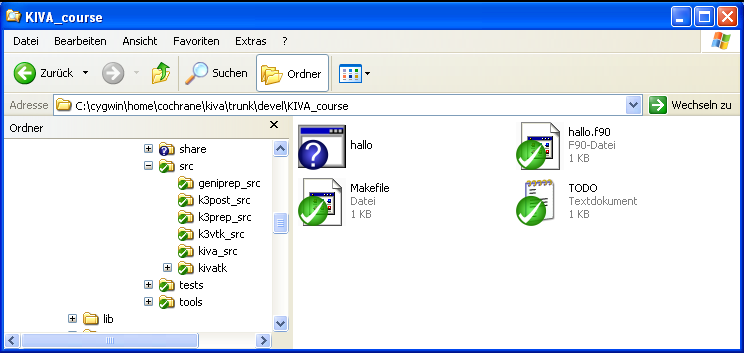
\includegraphics[width=0.5\textwidth]{windows_images/hallo_unknown_file.png}
    \end{center}
\end{frame}

%%%%%%%%%%%%%%%%%%%%%%%%%%%%%%%%%%%%%%%%%%%%%%%%%%%%%%%%%%%%%%%%%%%%%%%%%%%%
\begin{frame}[fragile]
    \frametitle{Properties---Ignoring files (cont.)}

    We can ignore this file, so that it doesn't appear with the question
    mark:
    \begin{itemize}
        \item Right-click on the file
        \item Select \ttt{TortoiseSVN} $\rightarrow$
            \ttt{Add to ignore list} $\rightarrow$ \ttt{hallo.exe}
    \end{itemize}
    Now the file icon no longer contains a blue question mark.

    \begin{center}
        \begin{tabularx}{\textwidth}{cX}
            %\imagetop{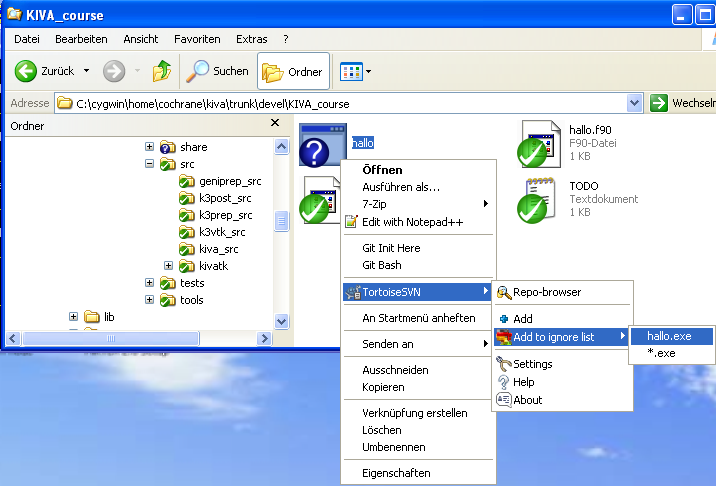
\includegraphics[width=0.4\textwidth]{windows_images/hallo_file_add_ignore_list.png}}
            &
            %\imagetop{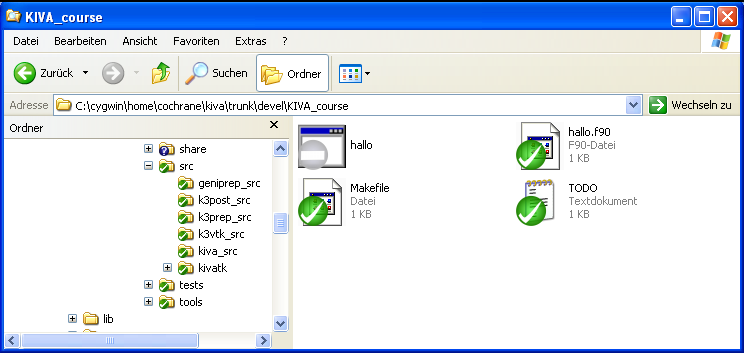
\includegraphics[width=0.5\textwidth]{windows_images/hallo_file_ignored_precommit.png}}
        \end{tabularx}
    \end{center}
\end{frame}

%%%%%%%%%%%%%%%%%%%%%%%%%%%%%%%%%%%%%%%%%%%%%%%%%%%%%%%%%%%%%%%%%%%%%%%%%%%%
\begin{frame}[fragile]
    \frametitle{Properties---Ignoring files (cont.)}

    This is a change which needs to be checked in, thus we commit the
    change as usual:
    \begin{itemize}
        \item Right-click in the directory
        \item Select \ttt{SVN Commit...}
    \end{itemize}

    \begin{center}
        %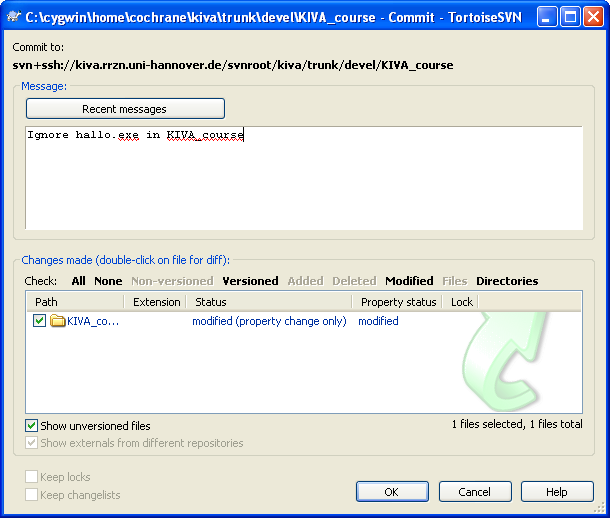
\includegraphics[width=0.4\textwidth]{windows_images/hallo_file_ignore_commit.png}
    \end{center}
\end{frame}


%%%%%%%%%%%%%%%%%%%%%%%%%%%%%%%%%%%%%%%%%%%%%%%%%%%%%%%%%%%%%%%%%%%%%%%%%%%%
\begin{frame}[fragile]
    \frametitle{Properties---Windows and Unix working together}
    \linuxframe

    \begin{itemize}
        \item Line endings in text files on Windows end with CRLF
        \item Line endings in text files on Unix end with CR
    \end{itemize}

    On Linux, Windows text files contain a \ttalert{\^{}M} character at the
    end of each line.  On Windoes, Linux text files seem to contain just the
    one line!  This is unless your editor is clever.  The
    \ttalert{svn:eol-style} Subversion property maintains peace between the
    Windows and Linux worlds.
    \ttalert{svn propset svn:eol-style <style> <file>}.

    \begin{description}
        \item[\ttalert{svn:eol-style native}] For CRLF on Windows and only
            CR on Unix.
        \item[\ttalert{svn:eol-style CRLF}] If only CRLF is desired.
        \item[\ttalert{svn:eol-style CR}] If only CR is desired.
        \item[\ttalert{svn:eol-style LF}] If only LF is desired.
\end{description}

\begin{lstlisting}
$ svn ps svn:eol-style native hallo.c
property 'svn:eol-style' set on 'hallo.c'
\end{lstlisting}
\end{frame}

%%%%%%%%%%%%%%%%%%%%%%%%%%%%%%%%%%%%%%%%%%%%%%%%%%%%%%%%%%%%%%%%%%%%%%%%%%%%
\begin{frame}[fragile]
    \frametitle{Properties---Windows and Unix working together (cont.)}
    \linuxframe

    These changes of course change the file; not the file's contents, but
    the property.  This is why \ttalert{svn status} shows that the file was
    modified, but this time in the \emph{second} column.

\begin{lstlisting}
$ svn st
 M     hallo.c
\end{lstlisting}

    As one would expect, these changes should be committed:
\begin{lstlisting}
$ svn ci -m "Set EOL style to native" hallo.c
Sending        hallo.c

Committed revision 10.
\end{lstlisting}
\end{frame}

%%%%%%%%%%%%%%%%%%%%%%%%%%%%%%%%%%%%%%%%%%%%%%%%%%%%%%%%%%%%%%%%%%%%%%%%%%%%
\begin{frame}[fragile]
    \frametitle{Properties---Executable files}
    \linuxframe

    Perl, Python, Shell (etc.) scripts are often directly executable.
    One can set this behaviour in Unix with the \ttalert{chmod} command.
    Subversion, however, still sees these files as text files.
    Nevertheless, one would like these files to be executable even when the
    working copy is freshly checked out.  Therefore one sets the
    \ttalert{svn:executable} property on such files.

    \ttalert{svn propset svn:executable <on/off> <filename>}

\begin{lstlisting}
$ svn ps svn:executable on hallo.pl 
property 'svn:executable' set on 'hallo.pl'
$ ls -l hallo.pl 
-rwxr-xr-x 1 cochrane cochrane 65 2010-09-18 16:31 hallo.pl
$ svn ci -m "Set the executable bit" hallo.pl 
Sending        hallo.pl

Committed revision 12.
$  ./hallo.pl 
Moin!
\end{lstlisting}
\end{frame}

%%%%%%%%%%%%%%%%%%%%%%%%%%%%%%%%%%%%%%%%%%%%%%%%%%%%%%%%%%%%%%%%%%%%%%%%%%%%
\begin{frame}[fragile]
    \frametitle{Properties---Binary files}
    \linuxframe

    Usually Subversion notices correctly whether or not a file contains
    plain text or binary data.  Sometimes it doesn't get this right.  PDF
    files are a common example.  In this case one can explicitly set the
    \ttalert{svn:mime-type} property.

\ttalert{svn propset svn:mime-type <MIME description>}

\begin{lstlisting}
$ svn add hallo.png hallo.svg hallo.pdf
A  (bin)  hallo.png
A         hallo.svg
A         hallo.pdf
\end{lstlisting}

    In this case we want the PDF file to be kept under version control (the
    file will be changed at some stage and the history of these changes is
    important to us) however Subversion didn't (automatically) notice that
    the file contains binary data.
\end{frame}

%%%%%%%%%%%%%%%%%%%%%%%%%%%%%%%%%%%%%%%%%%%%%%%%%%%%%%%%%%%%%%%%%%%%%%%%%%%%
\begin{frame}[fragile]
    \frametitle{Properties---Binary files}
    \linuxframe

    Hence we need to set the \ttalert{svn:mime-type} property:
\begin{lstlisting}
$ svn ps svn:mime-type application/octet-stream hallo.pdf
property 'svn:mime-type' set on 'hallo.pdf'
$ svn ci
Adding  (bin)  trunk/hallo.pdf
Adding  (bin)  trunk/hallo.png
Adding         trunk/hallo.svg
Transmitting file data ...
Committed revision 13.
\end{lstlisting}
    Now Subversion knows about the file's binary nature and is correctly
    checked in.
\end{frame}

%%%%%%%%%%%%%%%%%%%%%%%%%%%%%%%%%%%%%%%%%%%%%%%%%%%%%%%%%%%%%%%%%%%%%%%%%%%%
\begin{frame}[fragile]
    \frametitle{Properties---Automatic keywords}
    \linuxframe

    In some software development projects it is common practice that each
    file contain the author, revision and date of the last change to the
    file.  This can be set automatically in Subversion via certain keywords
    and the use of the \ttalert{svn:keywords} property.

    Let's add the following lines to \ttalert{hallo.c}:
\begin{lstlisting}
// $Id$
// $Author$
// $Revision$
// $Date$
\end{lstlisting}
    This doesn't change anything for Subversion (other than that the file
    has now been changed).  CVS, however, interprets these lines straight
    away; sometimes this isn't what one wants!  In Subversion, when one
    wants to use these keywords, one needs to activate the
    \ttalert{svn:keywords} property.

\begin{lstlisting}
$ svn ps svn:keywords "Author Revision Date" hallo.c
property 'svn:keywords' set on 'hallo.c'
\end{lstlisting}
\end{frame}

%%%%%%%%%%%%%%%%%%%%%%%%%%%%%%%%%%%%%%%%%%%%%%%%%%%%%%%%%%%%%%%%%%%%%%%%%%%%
\begin{frame}[fragile]
    \frametitle{Properties---Automatic keywords (cont.)}
    \linuxframe
    \vspace*{-3mm}
    We've changed both content and properties, thus we now see an
    \ttalert{M} in the first two columns in the \ttalert{svn status} output:
\begin{lstlisting}[basicstyle=\tiny\ttfamily\color{black}]
$ svn st
MM     hallo.c
\end{lstlisting}

    A \ttalert{svn diff} also shows us what was changed:
\begin{lstlisting}[basicstyle=\tiny\ttfamily\color{black}]
$ svn di
Index: hallo.c
===================================================================
--- hallo.c (revision 10)
+++ hallo.c (working copy)
@@ -1,4 +1,8 @@
 // hallo: a program to say "hallo!"
+// $Id$
+// $Author$
+// $Revision$
+// $Date$
 #include <stdio.h>
 
 int main(void) {

Property changes on: hallo.c
___________________________________________________________________
Added: svn:keywords
   + Author Revision Date
\end{lstlisting}
\end{frame}

%%%%%%%%%%%%%%%%%%%%%%%%%%%%%%%%%%%%%%%%%%%%%%%%%%%%%%%%%%%%%%%%%%%%%%%%%%%%
\begin{frame}[fragile]
    \frametitle{Properties---Automatic keywords (cont.)}
    \linuxframe

    Where are these magical automatic keywords?  They only turn up after one
    has checked in the file.
\begin{lstlisting}[basicstyle=\tiny\ttfamily\color{black}]
$ svn ci
Sending        trunk/hallo.c
Transmitting file data .
Committed revision 14.
$ cat hallo.c
// hallo: a program to say "hallo!"
// $Id$
// $Author: vcskurs15 $
// $Revision: 14 $
// $Date: 2010-09-18 17:26:56 +0200 (Sat, 18 Sep 2010) $
\end{lstlisting}

    Where is the keyword for \ttalert{Id}?  This wasn't set and is therefore
    not expanded.  To be honest, in most cases the \ttalert{Id} keyword is
    all that is needed, since this is a simply a compact version containing
    the other keywords mentioned above.
\end{frame}

%%%%%%%%%%%%%%%%%%%%%%%%%%%%%%%%%%%%%%%%%%%%%%%%%%%%%%%%%%%%%%%%%%%%%%%%%%%%
\begin{frame}[fragile]
    \frametitle{Properties---Automatic keywords (cont.)}
    \linuxframe
    \vspace*{-3mm}
    Let's delete the unnecessary files and correct the
    \ttalert{svn:keywords} property:

\begin{lstlisting}[basicstyle=\tiny\ttfamily\color{black}]
$ vim hallo.c
$ svn ps svn:keywords "Id" hallo.c
property 'svn:keywords' set on 'hallo.c'
$ svn di
Index: hallo.c
===================================================================
--- hallo.c (revision 14)
+++ hallo.c (working copy)
@@ -1,8 +1,5 @@
 // hallo: a program to say "hallo!"
 // $Id$
-// $Author$
-// $Revision$
-// $Date$
 #include <stdio.h>

 int main(void) {
Property changes on: hallo.c
___________________________________________________________________
Modified: svn:keywords
   - Author Revision Date
   + Id
\end{lstlisting}
    The old properties have been deleted and only \ttalert{Id} has been
    added and one can see this with \ttalert{svn diff}.  Cool!
\end{frame}

%%%%%%%%%%%%%%%%%%%%%%%%%%%%%%%%%%%%%%%%%%%%%%%%%%%%%%%%%%%%%%%%%%%%%%%%%%%%
\begin{frame}[fragile]
    \frametitle{Properties---Automatic keywords (cont.)}
    \linuxframe

    We now check in the file and the \ttalert{Id} keyword is expanded as we
    expect:
\begin{lstlisting}
$ svn ci -m "Only the Id keyword is needed" hallo.c
Sending        hallo.c
Transmitting file data .
Committed revision 15.
$ cat hallo.c
// hallo: a program to say "hallo!"
// $Id: hallo.c 15 2010-09-18 15:31:47Z vcskurs15 $
\end{lstlisting}

\end{frame}

%%%%%%%%%%%%%%%%%%%%%%%%%%%%%%%%%%%%%%%%%%%%%%%%%%%%%%%%%%%%%%%%%%%%%%%%%%%%
\begin{frame}[fragile]
\frametitle{Properties---Sundry properties}

    It is possible to do more than just edit and set properties.  One can
    also delete them get them and list them.

    \begin{description}
        \item[propedit] Edit the property
        \item[propset] Set the property
        \item[propdel] Delete the property
        \item[propget] Get the property
        \item[proplist] List all properties in a file
    \end{description}

\begin{lstlisting}
$ svn propget svn:mime-type hallo.png
application/octet-stream
\end{lstlisting}

\begin{lstlisting}
$ svn proplist hallo.c
Properties on 'hallo.c':
  svn:keywords
  svn:mergeinfo
  svn:eol-style
$ svn propget svn:eol-style hallo.c
native
\end{lstlisting}

\end{frame}

%%%%%%%%%%%%%%%%%%%%%%%%%%%%%%%%%%%%%%%%%%%%%%%%%%%%%%%%%%%%%%%%%%%%%%%%%%%%
\subsection{Branches, Tags and Merging}
\begin{frame}[fragile,label=branch-merge]
    \frametitle{Branches, Tags and Merging}

    One of the most powerful features of version control systems is the
    possibility to have multiple parallel development directions and to be
    able to manage them all within the one system.

    For example:
    \begin{description}
        \item[Feature branches:] for the development of new features
            \begin{itemize}
                \item don't disturb other lines of development
                \item one can see the changes which take place and give
                    feedback
                \item usually only have a short lifespan
            \end{itemize}
        \item[Maintenance branches:] long term maintenance of software
        \begin{itemize}
            \item bugs (found and corrected in the maintenance branch)
                can be merged with trunk
            \item bugs (found and corrected in trunk) can be merged into
                the maintenance branch
            \item are not as static as a tag (from the human point of view)
        \end{itemize}
    \end{description}
\end{frame}

%%%%%%%%%%%%%%%%%%%%%%%%%%%%%%%%%%%%%%%%%%%%%%%%%%%%%%%%%%%%%%%%%%%%%%%%%%%%
\begin{frame}[fragile]
    \frametitle{Branches, Tags and Merging (cont.)}
    How one uses branches is basically a question of project policy.  For
    example:
    \begin{itemize}
        \item Branches are \enquote{stable}; trunk is only for development
        \item Trunk is \enquote{stable}; branches are only for development
    \end{itemize}

\begin{center}
    \resizebox{\textwidth}{!}{
        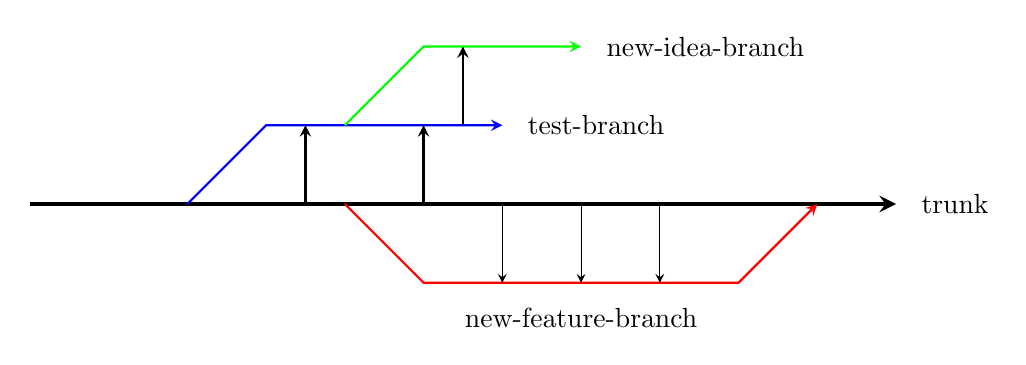
\begin{tikzpicture}
% trunk
\node at (11.2,0) [anchor=west] {trunk};
\draw [->,ultra thick,>=stealth] (0,0) -- (11,0);
% upper branch
\node at (6.2,1) [anchor=west] {test-branch};
\draw [->,thick,>=stealth,color=blue] (2,0) -- (3,1) -- (6,1);
\draw [->,thick,>=stealth] (3.5,0) -- (3.5,1);
\draw [->,thick,>=stealth] (5,0) -- (5,1);
% upper-upper branch
\node at (7.2,2) [anchor=west] {new-idea-branch};
\draw [->,thick,>=stealth,color=green] (4,1) -- (5,2) -- (7,2);
\draw [->,thick,>=stealth] (5.5,1) -- (5.5,2);
% lower branch
\node at (7,-1.2) [anchor=north] {new-feature-branch};
\draw [->,thick,>=stealth,color=red] (4,0) -- (5,-1) -- (9,-1) -- (10,0);
\draw [->,>=stealth] (6,0) -- (6,-1);
\draw [->,>=stealth] (7,0) -- (7,-1);
\draw [->,>=stealth] (8,0) -- (8,-1);
\end{tikzpicture}

    }
\end{center}

\end{frame}

%%%%%%%%%%%%%%%%%%%%%%%%%%%%%%%%%%%%%%%%%%%%%%%%%%%%%%%%%%%%%%%%%%%%%%%%%%%%
\begin{frame}[fragile]
    \frametitle{Branches, Tags and Merging (cont.)}
    \linuxframe

    In Subversion, new branches are created via a copy operation:

    \ttalert{svn copy <source url> <target url> -m "<comment>"}

    This only happens on the server; one then merely needs to check out the
    new branch via either \ttalert{svn checkout} or \ttalert{svn update}.

\begin{lstlisting}[basicstyle=\tiny\ttfamily\color{black}]
$ svn copy \
svn+ssh://vcskurs15@host.name/svnroot/projects/hallo/trunk \
svn+ssh://vcskurs15@host.name/svnroot/projects/hallo/branches/test-branch

Committed revision 16.
\end{lstlisting}

\vspace*{-3mm}

\ttalert{svn checkout}
\begin{lstlisting}[basicstyle=\tiny\ttfamily\color{black}]
$ svn co
svn+ssh://vcskurs15@host.name/svnroot/projects/hallo/branches/test-branch
hallo_test-branch
A    hallo_test-branch/hallo.c
A    hallo_test-branch/hallo.png
A    hallo_test-branch/TODO
A    hallo_test-branch/hallo.pdf
A    hallo_test-branch/hallo.pl
A    hallo_test-branch/Makefile
A    hallo_test-branch/hallo.svg
 U   hallo_test-branch
Checked out revision 16. 
\end{lstlisting}
\end{frame}

%%%%%%%%%%%%%%%%%%%%%%%%%%%%%%%%%%%%%%%%%%%%%%%%%%%%%%%%%%%%%%%%%%%%%%%%%%%%
\begin{frame}[fragile]
    \frametitle{Branches, Tags and Merging (cont.)}
    \linuxframe

\ttalert{svn update}
\begin{lstlisting}[basicstyle=\tiny\ttfamily\color{black}]
$ svn up
A    branches/test-branch
A    branches/test-branch/hallo.c
A    branches/test-branch/hallo.png
A    branches/test-branch/TODO
A    branches/test-branch/hallo.pdf
A    branches/test-branch/hallo.pl
A    branches/test-branch/Makefile
A    branches/test-branch/hallo.svg
Updated to revision 16.
\end{lstlisting}

\end{frame}

%%%%%%%%%%%%%%%%%%%%%%%%%%%%%%%%%%%%%%%%%%%%%%%%%%%%%%%%%%%%%%%%%%%%%%%%%%%%
\begin{frame}[fragile]
    \frametitle{Branches, Tags and Merging (cont.)}

    \begin{alertblock}{Tags}

        Tags are basically only things for people.  The operation in
        Subversion is identical to creation of a branch, the difference is
        in how a human being considers a tag or a branch (tags, branches and
        trunk are really just directories).  A branch is more often seen as
        something which has a limited lifetime, since the development will
        flow back into the trunk at some point (at which point the branch
        ends) or the development is seen as unnecessary and stops.  A tag is
        often used for \enquote{software releases} (e.g.~version 0.1, 0.2
        etc.) and is therefore much more permanent.

    \end{alertblock}
\end{frame}

%%%%%%%%%%%%%%%%%%%%%%%%%%%%%%%%%%%%%%%%%%%%%%%%%%%%%%%%%%%%%%%%%%%%%%%%%%%%
\begin{frame}[fragile]
    \frametitle{Branches, Tags and Merging (cont.)}
    \linuxframe

    \begin{alertblock}{\enquote{Tagging a release}}
\begin{lstlisting}[basicstyle=\tiny\ttfamily\color{black}]
$ svn copy\
svn+ssh://vcskurs15@host.name/svnroot/projects/hallo/trunk\
svn+ssh://vcskurs15@host.name/svnroot/projects/hallo/tags/hallo_version_1.0\
-m "Tagging version 1.0"

Committed revision 17.
\end{lstlisting}
    \end{alertblock}

\end{frame}

%%%%%%%%%%%%%%%%%%%%%%%%%%%%%%%%%%%%%%%%%%%%%%%%%%%%%%%%%%%%%%%%%%%%%%%%%%%%
\begin{frame}[fragile]
    \frametitle{Branches, Tags and Merging (cont.)}

    \begin{alertblock}{Merging}
        When the main development happens in trunk and branches are
        \enquote{feature branches}, then it's a good idea that when one
        works on a branch, that the latest changes from trunk are
        periodically \enquote{merged} into your branch.  This reduces the
        risk that the branch development wanders too far away from the trunk
        development which would cause difficulties when the branch is to be
        merged back into the trunk at some later time.

        Since version 1.5, Subversion remembers which merges from trunk have
        already happened and so only pulls in the latest changes when the
        next merge takes place.  This is important when a branch is to be
        merged back into trunk: the previous changes on trunk shouldn't be
        played back onto the trunk!

    \end{alertblock}
\end{frame}

%%%%%%%%%%%%%%%%%%%%%%%%%%%%%%%%%%%%%%%%%%%%%%%%%%%%%%%%%%%%%%%%%%%%%%%%%%%%
\begin{frame}[fragile]
    \frametitle{Branches, Tags and Merging (cont.)}
    \linuxframe

    As an example of merging, we can use the \ttalert{hallo\_test-branch} in
    order to reproduce the functionality of the C program in Perl.
\begin{multicols}{2}
\begin{lstlisting}[basicstyle=\tiny\ttfamily\color{black}]
$ svn di
Index: hallo.pl
=============================================
--- hallo.pl    (revision 16)
+++ hallo.pl    (working copy)
@@ -3,4 +3,14 @@
 use strict;
 use warnings;
 
-print "Moin!\n";
+# north
+print "Moin, moin!\n";
+# middle
+print "Tach!\n";
+print "Halli hallo!\n";
+# south
+print "Gruess Gott!\n";
+# further south
+print "Gruetzi!\n";
+# even further south...
+print "Gudday, mate!\n";
\end{lstlisting}
\columnbreak
\begin{lstlisting}[basicstyle=\tiny\ttfamily\color{black}]
$ ./hallo.pl
Moin, moin!
Tach!
Halli hallo!
Gruess Gott!
Gruetzi!
Gudday, mate!
$ svn ci -m "Perl copycats C"
Sending        hallo.pl
Transmitting file data .
Committed revision 18.
\end{lstlisting}
\end{multicols}
\end{frame}

%%%%%%%%%%%%%%%%%%%%%%%%%%%%%%%%%%%%%%%%%%%%%%%%%%%%%%%%%%%%%%%%%%%%%%%%%%%%
\begin{frame}[fragile]
    \frametitle{Branches, Tags and Merging (fort.)}
    \linuxframe

    The development on trunk continues\ldots
\begin{lstlisting}[basicstyle=\tiny\ttfamily\color{black}]
$ svn log
------------------------------------------------------------------------
r21 | vcskurs15 | 2010-09-18 20:49:34 +0200 (Sat, 18 Sep 2010) | 2 lines

hallo.py is now executable

------------------------------------------------------------------------
r20 | vcskurs15 | 2010-09-18 20:48:30 +0200 (Sat, 18 Sep 2010) | 2 lines

The Makefile is no longer necessary

------------------------------------------------------------------------
r19 | vcskurs15 | 2010-09-18 20:47:48 +0200 (Sat, 18 Sep 2010) | 2 lines

C is silly.  Development now takes place in Python
\end{lstlisting}

We now pull the changes in trunk into the branch\ldots
\begin{lstlisting}[basicstyle=\tiny\ttfamily\color{black}]
$ svn merge \
svn+ssh://vcskurs15@host.name/svnroot/projects/hallo/trunk
--- Merging r16 through r21 into '.':
A    hallo.py
D    hallo.c
D    Makefile
\end{lstlisting}
\end{frame}

%%%%%%%%%%%%%%%%%%%%%%%%%%%%%%%%%%%%%%%%%%%%%%%%%%%%%%%%%%%%%%%%%%%%%%%%%%%%
\begin{frame}[fragile]
    \frametitle{Branches, Tags and Merging (fort.)}
    \linuxframe

    and we can continue working.
\begin{lstlisting}[basicstyle=\tiny\ttfamily\color{black}]
$ svn st
 M     .
D      hallo.c
A  +   hallo.py
M      hallo.pl
D      Makefile
$ svn ci -m "More flexible?"
Sending        .
Deleting       Makefile
Deleting       hallo.c
Sending        hallo.pl
Adding         hallo.py
Transmitting file data .
Committed revision 22.
$ svn ci -m "Definitely more flexible"
Sending        hallo.pl
Transmitting file data .
Committed revision 23.
\end{lstlisting}
\end{frame}

%%%%%%%%%%%%%%%%%%%%%%%%%%%%%%%%%%%%%%%%%%%%%%%%%%%%%%%%%%%%%%%%%%%%%%%%%%%%
\begin{frame}[fragile]
    \frametitle{Branches, Tags and Merging (cont.)}
    \linuxframe
    \vspace*{-3mm}

    We are now ready to merge our changes back \emph{into} the trunk and so
    merge \emph{from} trunk one last time

\begin{lstlisting}[basicstyle=\tiny\ttfamily\color{black}]
$ svn merge\
svn+ssh://vcskurs15@host.name/svnroot/projects/hallo/trunk
--- Merging r22 through r24 into '.':
U    hallo.py
$ svn up   # we should now be up to date...
At revision 24.
$ svn st
 M     .
M      hallo.py
$ svn ci -m "Pulled in latest changes from trunk"
Sending        .
Sending        hallo.py
Transmitting file data .
Committed revision 25.
\end{lstlisting}

    We can now merge our branch with trunk
\begin{lstlisting}[basicstyle=\tiny\ttfamily\color{black}]
$ cd hallo_gemeinsam/trunk
$ svn up   # we need to be up to date...
$ svn merge --reintegrate
svn+ssh://vcskurs15@host.name/svnroot/projects/hallo/branches/test-branch
--- Merging differences between repository URLs into '.':
U    hallo.pl
 U   .
\end{lstlisting}

\end{frame}

%%%%%%%%%%%%%%%%%%%%%%%%%%%%%%%%%%%%%%%%%%%%%%%%%%%%%%%%%%%%%%%%%%%%%%%%%%%%
\begin{frame}[fragile]
    \frametitle{Branches, Tags and Merging (cont.)}
    \linuxframe

    Let's commit once more
\begin{lstlisting}[basicstyle=\tiny\ttfamily\color{black}]
$ svn st
 M     .
M      hallo.pl
$ svn ci -m "merged test-branch with trunk"
Sending        trunk
Sending        trunk/hallo.pl
Transmitting file data .
Committed revision 26.
\end{lstlisting}

We no longer need the test branch since the changes have been merged with
trunk.  We can now simply delete the branch (the branch's history is still in
the repository).
\begin{lstlisting}[basicstyle=\tiny\ttfamily\color{black}]
$ svn delete
svn+ssh://vcskurs15@host.name/svnroot/projects/hallo/branches/test-branch
-m "Delte the test branch"

Committed revision 27.
\end{lstlisting}

\end{frame}

%%%%%%%%%%%%%%%%%%%%%%%%%%%%%%%%%%%%%%%%%%%%%%%%%%%%%%%%%%%%%%%%%%%%%%%%%%%%
\begin{frame}{Exercise---Development with branches}
    \begin{itemize}
        \item Check out the \ttalert{hallo} project
        \item Start a new branch
        \item Possible topics of development:
        \begin{itemize}
            \item random greetings
            \item a menu system
            \item greetings in different languages from different countries
                and regions
            \item surprise me!
        \end{itemize}
    \end{itemize}
\end{frame}

%%%%%%%%%%%%%%%%%%%%%%%%%%%%%%%%%%%%%%%%%%%%%%%%%%%%%%%%%%%%%%%%%%%%%%%%%%%%
\subsection{Extras}
\begin{frame}[fragile]
    \frametitle{Extra Subversion features and topics}
    \linuxframe

    \begin{itemize}
        \item Find out who changed which lines and in which revisions:
            \ttalert{svn blame <filename>}; also \ttalert{praise}, \ttalert{annotate}
        \item Export a project without the \ttalert{.svn} directories;
            e.g.~when one does a release: \ttalert{svn export}
        \item File locking: \ttalert{svn lock}, \ttalert{svn unlock}
        \item Send emails with each commit: commit hooks; happens on the
            server and is configured by the system administrator in the
            \ttalert{post-commit} file
        \item Automatically pull changes from other projects:
            the \ttalert{svn:external} property 
        \item If one has changed many files which belong to different ideas,
            it is possible to label these files with the name of the idea.
            This is the concept of a \emph{changeset} and is set up using
            the \ttalert{changelist} command:
            \ttalert{svn changelist <changelist name> <files...>}
        \end{itemize}

\end{frame}

%%%%%%%%%%%%%%%%%%%%%%%%%%%%%%%%%%%%%%%%%%%%%%%%%%%%%%%%%%%%%%%%%%%%%%%%%%%%
\begin{frame}[fragile]
\frametitle{Changing a repository's name}

Sometimes one wants to change the name of the repository as it no longer
properly reflects its purpose anymore.  To do this the administrator of the
Subversion repository merely needs to change the name of the base directory
containing the repository:
\begin{lstlisting}
cd /svnroot/...
mv <oldreponame> <newreponame>
\end{lstlisting}

The users now need to update their working copies.  They do this with the
\ttalert{svn switch} command:
\begin{lstlisting}
svn switch --relocate <old_repo_url> <new_repo_url>
\end{lstlisting}

For example:
\begin{lstlisting}
svn switch --relocate \
    svn+ssh://vcskurs15@host.name/svnroot/projects/hallo \
    svn+ssh://vcskurs15@host.name/svnroot/projects/moin
\end{lstlisting}
\end{frame}

%%%%%%%%%%%%%%%%%%%%%%%%%%%%%%%%%%%%%%%%%%%%%%%%%%%%%%%%%%%%%%%%%%%%%%%%%%%%
\subsection{Resources}
\begin{frame}{Resources}
    \begin{itemize}
        \item The Subversion book
            \begin{itemize}
                \item O'Reilly Media
                \item \url{http://svnbook.red-bean.com}
            \end{itemize}
        \item Subversion web site:
            \url{http://subversion.tigris.org}
        \item TortoiseSVN; Subversion for Windows:
            \url{http://tortoisesvn.tigris.org}
        \item Wikipedia:
            \url{http://en.wikipedia.org/wiki/Apache_Subversion}
    \end{itemize}
\end{frame}

% vim: expandtab shiftwidth=4:


%%%%%%%%%%%%%%%%%%%%%%%%%%%%%%%%%%%%%%%%%%%%%%%%%%%%%%%%%%%%%%%%%%%%%%%%%%%%
\begin{frame}{Thank you!}
\begin{center}
\huge
Many thanks for your attention!
\end{center}
\end{frame}

\end{document}

% vim: expandtab shiftwidth=4:
